%\newcommand{\notatki}{1}
\documentclass{sa}
\usepackage{array} %dla poziomego wyrownania (m) w tabeli
\usepackage{soul}

\newcommand{\ang}[1]{(ang. \emph{#1})}
\renewcommand{\vec}[1]{\ensuremath\mathbf{#1}}
\newcommand{\grad}{\ensuremath\nabla}
\let\avg\overline

\usetikzlibrary{datavisualization}
\usetikzlibrary{datavisualization.formats.functions}

\usepackage{hyperref}
\graphicspath{{01_wstep/}}
\subtitle{Uwagi organizacyjne}
\begin{document}
\begin{frame}
\titlepage
\end{frame}
\begin{frame}{Kontakt}
mgr inż. Jędrzej Potoniec \\
\url{Jedrzej.Potoniec@cs.put.poznan.pl}\\
\url{http://www.cs.put.poznan.pl/jpotoniec}
\url{https://github.com/jpotoniec/sa}
\end{frame}
\begin{frame}{Zasady oceniania}
\begin{description}
\item[wykład] test wielokrotnego wyboru
\item[laboratoria] wykonanie ćwiczeń laboratoryjnych
\end{description}
\end{frame}
\begin{frame}{Skala ocen}
\begin{center}
\begin{tabular}{l|r}
\% punktów & ocena \\
\hline
$\left(-\infty; 50\right]$ & 2,0 \\
$\left(50; 60\right]$ & 3,0 \\
$\left(60; 70\right]$ & 3,5 \\
$\left(70; 80\right]$ & 4,0 \\
$\left(80; 90\right]$ & 4,5 \\
$\left(90; \infty\right)$ & 5,0 \\
\end{tabular}
\end{center}
\end{frame}
%\begin{frame}{Obecność}
%\begin{block}{Regulamin studiów, rozdział II, par.9 pkt. 11}
%Uczestnictwo w zajęciach objętych planem studiów jest obowiązkowe dla nauczycieli akademickich i~studentów.
%Uczestnictwo w ćwiczeniach, zajęciach laboratoryjnych, projektowych, seminariach, pracowniach, lektoratach i~zajęciach WF jest kontrolowane przez prowadzącego.
%\end{block}
%{\tiny Regulamin studiów stacjonarnych i niestacjonarnych pierwszego i drugiego stopnia uchwalony przez Senat Akademicki Politechniki Poznańskiej Uchwała Nr 32/2016-2020 z dnia 29 marca 2017 r.
%}
%\end{frame}


\begin{frame}{Skąd nazwa?}
	\begin{block}{S. Russel, P. Norwig ,,Artificial Intelligence A Modern Approach'' (3ed)}
		An agent is anything that can be viewed as perceiving its environment throught sensors and acting upon that environment through actuators.
	\end{block}
\pause
	\begin{description}
		\item[człowiek] wzrok, słuch/ręce, nogi
		\item[robot] kamera, mikrofon/silniki
		\item[agent programowy] naciśnięcia klawiszy, odczyt plików/ekran, zapis plików
	\end{description}
\pause
	agent -- agenty, nie: \st{agent -- agenci}
\end{frame}

\begin{frame}{Literatura}
\begin{minipage}{.5\textwidth}
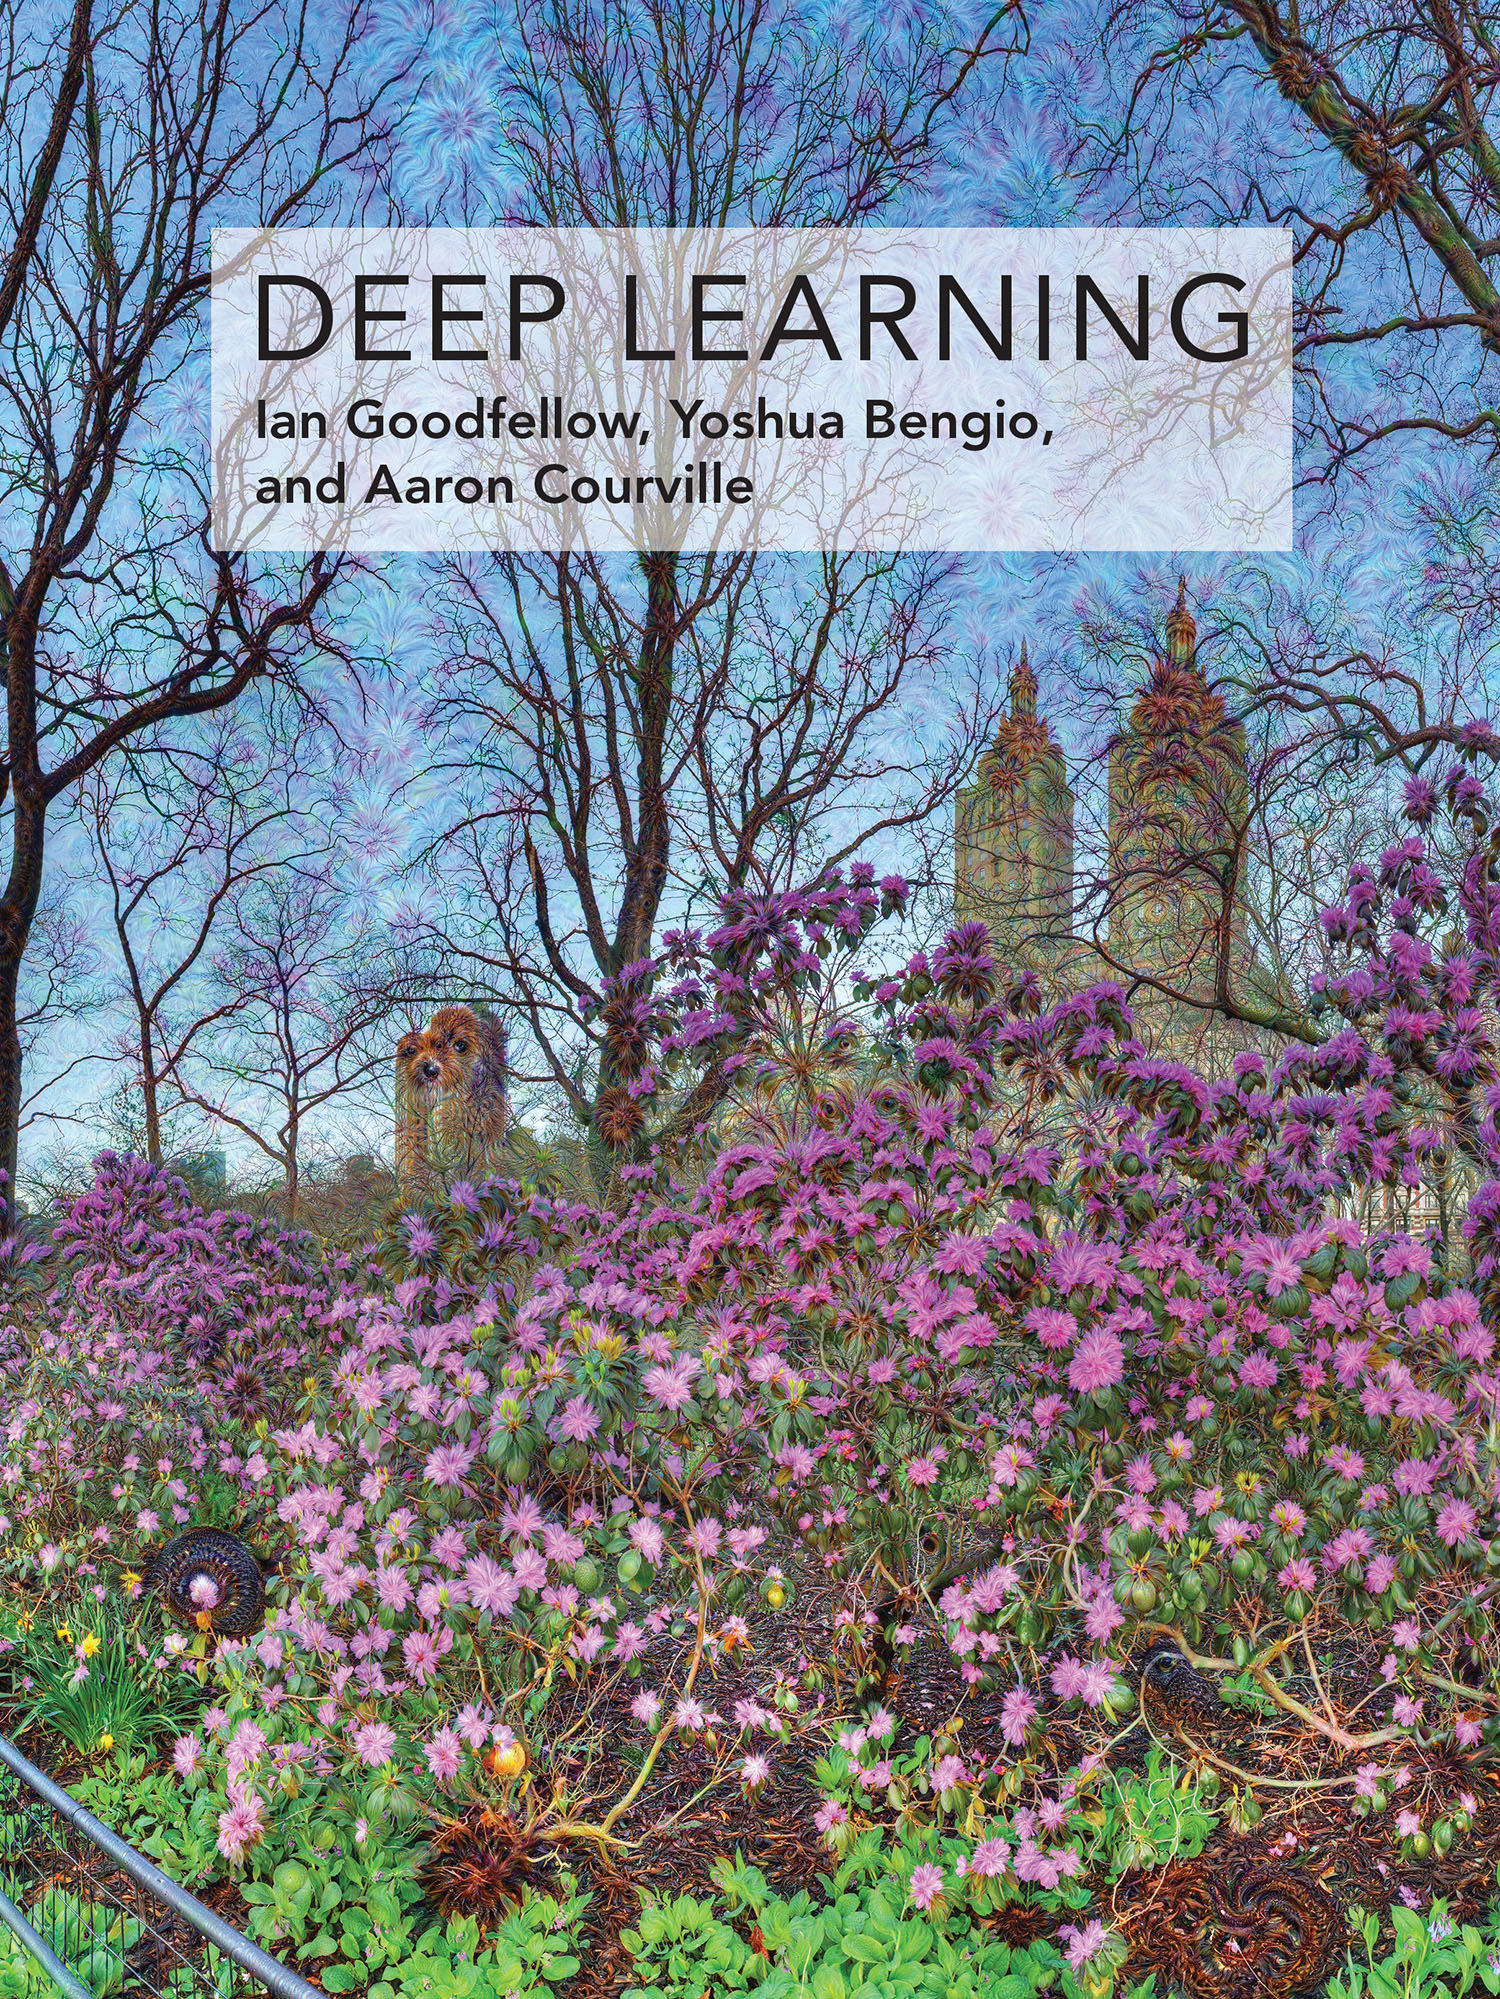
\includegraphics[width=\textwidth]{dl-book.jpg}
\end{minipage}
\begin{minipage}{.49\textwidth}
{\small I. Goodfellow, Y. Bengio, A. Courville}\\
\emph{Deep Learning}\\
MIT Press 2016 \\
\url{www.deeplearningbook.org}
\end{minipage}
\end{frame}
\begin{frame}{Literatura}
\begin{minipage}{.5\textwidth}
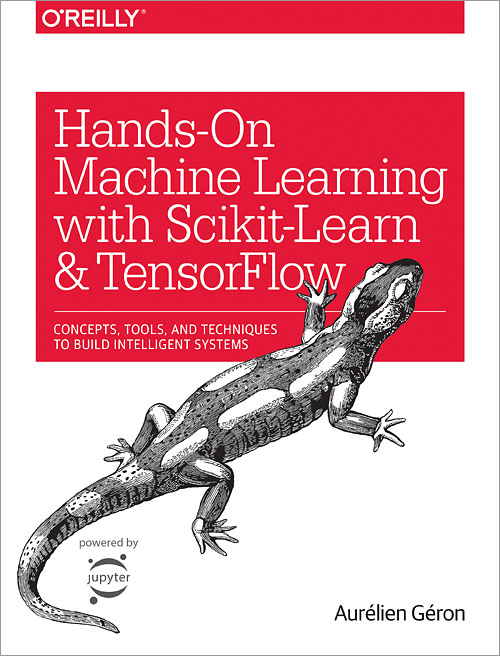
\includegraphics[width=\textwidth]{handson.jpg}
\end{minipage}
\begin{minipage}{.49\textwidth}
Aurélien Géron\\
\emph{Hands-On Machine Learning with Scikit-Learn and TensorFlow}\\
O'Reilly Media 2017
\end{minipage}
\end{frame}
\begin{frame}{Plan wykładu}
\begin{enumerate}
\item Regresja liniowa, wielomianowa i logistyczna
\item Warstwowe sieci neuronowe
\item Uczenie ze wzmocnieniem
\end{enumerate}
\end{frame}

\begin{frame}{Program uczący się}
\begin{block}{T. Mitchell \emph{Machine Learning} 1997}
Program komputerowy \emph{uczy się} z doświadczenia $E$ względem pewnej klasy zadań $T$ i miary jakości $P$, jeżeli wartość jego miary jakości $P$ na zadaniach z klasy $T$ poprawia się wraz ze ilością doświadczenia $E$.
\end{block}
\end{frame}

\begin{frame}{Niewyczerpująca lista klas zadań $T$}
\begin{itemize}
\item<+-> klasyfikacja
\item<+-> klasyfikacja z brakującymi wejściami
\item<+-> regresja
\item<+-> transkrypcja
\item<+-> tłumaczenie maszynowe
\item<+-> przewidywanie złożonych struktur
\item<+-> detekcja anomalii
\item<+-> synteza i próbkowanie
\item<+-> uzupełnianie brakujących wejść
\item<+-> usuwanie szumu
\item<+-> estymacja rozkładu prawdopodobieństwa
\end{itemize}
\end{frame}

\begin{frame}{Miary jakości $P$}
\begin{block}{}
Liczbowy sposób określenia jak dobrze/źle program rozwiązuje zadanie $T$.
\end{block}
%TODO zbiór uczący i testowy
%TODO inna miara w procesie uczenia, inna miara w procesie testowania
Bywa prosta do zdefiniowania i obiektywna, np. trafność klasyfikacji \ang{accuracy} w zadaniu \emph{jaka cyfra jest na rysunku}
\[ \frac{\text{odpowiedzi poprawne}}{\text{wszystkie odpowiedzi}} \]
%TODO podzielic na kilka slajdow, dolozyc przyklady nagryzmolonych cyfr
ale również nieobiektywna, np. trafność klasyfikacji w zadaniu \emph{czy ten pasażer jest terrorystą}
\[ \frac{\text{pasażerowie, którzy nie są terrorystami}}{\text{wszyscy pasażerowie}}\approx 100\% \]
albo trudna do zdefiniowania \emph{Grzegorz ma kota}
\begin{enumerate}
\item Grzegorz's got a cat
\item Grzegorz has a cat
\item He has a cat (Google Translate)
\item Gregory has a cat
\end{enumerate}
\end{frame}

\begin{frame}{Doświadczenie $E$}
\begin{itemize}
\item uczenie nadzorowane \ang{supervised}: zbiór przykładów opisanych cechami wraz z etykietami
\item uczenie nienadzorowane \ang{unsupervised}: zbiór przykładów opisanych cechami
\item uczenie ze wzmocnieniem \ang{reinforcement}: środowisko, w którym można wykonywać pewne akcje
\item uczenie częściowo nadzorowane \ang{semi-supervised}: niektóre przykłady mają etykiety
\end{itemize}
\end{frame}

\begin{frame}{Reprezentacja}
Macierz cech $\vec{X}$ mająca $n$ wierszy oraz $p$ kolumn, zwykle liczby rzeczywiste:
\[ \vec{X} = \begin{bmatrix}
X_{1,1} & X_{1,2} & \ldots & X_{1,p} \\
X_{2,1} & X_{2,2} & \ldots & X_{2,p} \\
\vdots & \vdots & \ddots & \vdots \\
X_{n,1} & X_{n,2} & \ldots & X_{n,p} \\
\end{bmatrix} \in \R^{n\times p} \]
\end{frame}

\begin{frame}{Reprezentacja}
Wektor etykiet $\vec{y}$
\[ \vec{y} = \begin{bmatrix}
y_1 \\
y_2 \\
\vdots \\
y_n
\end{bmatrix} \in \R^n \]
\end{frame}

\begin{frame}{Regresja liniowa}
Mając macierz cech $\vec{X}$ oraz wektor etyket $\vec{y}$ przewidzieć \alert{wektor parametrów} $\vec{w}$ tak, żeby błąd średniokwadratowy \ang{mean-square error (MSE)} był jak najmniejszy:
%TODO przykład
\begin{gather*}
MSE=\frac{1}{n}\sum_{i=1}^n (y_i-\hat{y_i})^2  \\
\hat{y_i}=\vec{w}^T\vec{X_i}  \\
\hat{\vec{y}} = \vec{X}\vec{w}
\end{gather*}
%TODO rozpisac mnozenie macierzy, zeby bylo widac ile jest y_i, moze zamiast umieszczac je na slajdach to policzyc na zajeciach?
\end{frame}

\begin{frame}{Regresja liniowa -- przypadek jednowymiarowy $p=1$}
$\vec{X}$ jest wektorem kolumnowym typu $n$, $w$ jest pojedynczą liczbą

\begin{gather*}
MSE=\frac{1}{n}\sum_{i=1}^n (y_i-wX_i)^2  \\
MSE \text{ jest najmniejsze} \iff \grad MSE = 0
\end{gather*}

Policzmy!

\note<1>{
\begin{gather*}
\grad MSE = \left(\frac{1}{n}\sum_{i=1}^n (y_i-wX_i)^2\right)' =
\frac{1}{n}\sum_{i=1}^n \left[ 2(y_i-wX_i)(-X_i) \right] = \\
\frac{2}{n}\sum_{i=1}^n \left[ X_i^2w-X_iy_i \right] =
\frac{2}{n} \left[\sum_{i=1}^n X_i^2w - \sum_{i=1}^nX_iy_i \right] = 0 \\
\sum_{i=1}^n X_i^2w - \sum_{i=1}^nX_iy_i = 0 \\
w\sum_{i=1}^n X_i^2 = \sum_{i=1}^nX_iy_i
w = \frac{\sum_{i=1}^nX_iy_i}{\sum_{i=1}^n X_i^2}
\end{gather*}
}
\end{frame}

\begin{frame}{Przykład}
Przewidzieć \alert{koszt paszy $y$} w zależności od \alert{liczby prosiaków $X$}

\begin{center}
%TODO zrobic tabele w pionie, zeby bylo spójnie
\begin{tabular}{l|rrr|rr}
$X$ & 4 & 7 & 9 & $w$ & $MSE$ \\
\hline
$y^{(1)}$ & 340 & 595 & 765 & \alert{?} & \alert{?} \\
\pause
$y^{(2)}$ & $348{,}5$ & $586{,}5$ & 765 & \alert{?} & \alert{?} \\
\pause
$y^{(3)}$ & 390 & 645 & 815 & \alert{?} & \alert{?} \\
\end{tabular}
%TODO rysunek prosiaka
\end{center}

\note<1>
{
\begin{itemize}
\item $y^{(1)}$: $w=85$, $mse=0$
\item $y^{(2)}$: niektóre prosiaki jedzą więcej niż inne
\item $y^{(3)}$: perfekcyjne prosiaki, ale dochodzą koszty wysyłki $w=91{.}85$ $MSE=4{,}34$
\end{itemize}
}
\end{frame}

\begin{frame}{Regresja liniowa -- przypadek jednowymiarowy $p=1$ z wyrazem wolnym}
$\vec{X}$ jest wektorem kolumnowym typu $n$, $w$ jest pojedynczą liczbą

\begin{gather*}
MSE=\frac{1}{n}\sum_{i=1}^n (y_i-wX_i-b)^2  \\
MSE \text{ jest najmniejsze} \iff \grad MSE = 0
\end{gather*}

\note<1>
{
Ze wzgl. na $w$: \[\sum_{i=1}^n \left[X_i^2-X_i(y-b)\right] = 0\]
Ze wzgl. na $b$: \[\sum_{i=1}^n \left[b-(y_i-X_iw)\right] = 0\]
Wyznaczamy $b$:
\[b=\frac{1}{n}\sum_{i=1}^n (y_i-X_iw) \]
Podstawiamy do pochodznej ze wzgl. na $w$:
\[\sum_{i=1}^n(X_i^2w-X_iy_i+\frac{1}{n}\sum_{i=1}^n (y_i-X_iw) \]
}
\note<2>
{
Po przekształceniu:
\[w=\frac{\sum_{i=1}^n X_i(y_i-\avg{\vec{y}})}{\sum_{i=1}^n X_i(X_i-\avg{\vec{X}})} \]
gdzie $\avg{\vec{y}}$ to średnia arytmetyczna $\vec{y}$
}
\end{frame}

\begin{frame}{Prosiaki}
Przewidzieć \alert{koszt paszy $y$} w zależności od \alert{liczby prosiaków $X$}

\begin{center}
\begin{tabular}{l|rrr|rrr}
$X$ & 4 & 7 & 9 & $w$ & $b$ & $MSE$ \\
\hline
$y^{(3)}$ & 390 & 645 & 815 & \alert{?} & \alert{?} & \alert{?} \\
\end{tabular}
%TODO rysunek prosiaka
\end{center}

\note<1>
{
\begin{itemize}
\item $y^{(3)}$: perfekcyjne prosiaki, ale dochodzą koszty wysyłki $w=85$, $b=50$, $MSE=0$
\end{itemize}
}
\end{frame}

\begin{frame}{Regresja liniowa -- wariant macierzowy}
\[ \vec{X} = \begin{bmatrix}
X_{1,1} & X_{1,2} & \ldots & X_{1,p} & \alert{1} \\
X_{2,1} & X_{2,2} & \ldots & X_{2,p} & \alert{1}\\
\vdots & \vdots & \ddots & \vdots & \alert{1}\\
X_{n,1} & X_{n,2} & \ldots & X_{n,p} & \alert{1}\\
\end{bmatrix} \in \R^{n\times (p\alert{+1})} \]

\pause
\[
\vec{X} = \begin{bmatrix}
4 & 1\\
7 & 1\\
9 & 1\\
\end{bmatrix}
\qquad
\vec{y}=\begin{bmatrix}
390 \\
645 \\
815 \\
\end{bmatrix}
\qquad
\vec{w}=\begin{bmatrix}
85 \\ 50
\end{bmatrix}
\]
\[
\hat{\vec{y}} = \vec{X}\vec{w}=\begin{matrix}
& \begin{bmatrix}
85 \\ 50
\end{bmatrix} \\
\begin{bmatrix}
4 & 1\\
7 & 1\\
9 & 1\\
\end{bmatrix}
&
\begin{bmatrix}
390 \\ 645 \\ 815
\end{bmatrix}
\end{matrix}
\]
\end{frame}

\begin{frame}{Regresja liniowa -- wariant macierzowy}
\[ MSE = \frac{1}{n}\left\|\vec{y}-\vec{X}\vec{w}\right\|^2_2=\frac{1}{n}\left(\vec{y}-\vec{X}\vec{w}\right)^T\left(\vec{y}-\vec{X}\vec{w}\right) \]
\[ \grad_\vec{w}MSE = 0 \]

Policzmy!

\note<1>
{
\begin{gather*}
\grad MSE \sim \grad \left(\vec{y}^T-\vec{w}^T\vec{X}^T\right)\left(\vec{y}-\vec{X}\vec{w}\right) = \\
\grad \left(\vec{y}^T\vec{y}-\vec{y}^T\vec{X}\vec{w}-\vec{w}^T\vec{X}^T\vec{y}+\vec{w}^T\vec{X}^T\vec{X}\vec{w}\right) =\\
\text{drugi i trzeci składnik to liczby, a do tego} (\vec{y}^T\vec{X}\vec{w})^T=\vec{w}^T\vec{X}^T\vec{y}  \\
\grad \left(\vec{y}^T\vec{y}-2\vec{y}^T\vec{X}\vec{w}+\vec{w}^T\vec{X}^T\vec{X}\vec{w}\right) =2\vec{y}^T\vec{X}-2\vec{w}^T\vec{X}^T\vec{X}=0\\
\vec{y}^T\vec{X} = \vec{w}^T\vec{X}^T\vec{X} \\
\vec{w}^T = \vec{y}^T\vec{X}\left(\vec{X}^T\vec{X}\right)^{-1} \\
\vec{w} = \left(\vec{X}^T\vec{X}\right)^{-1}\vec{X}^T\vec{y}
\end{gather*}
}
\end{frame}

\begin{frame}{Prosiaki}
\[\vec{w} = \left(\vec{X}^T\vec{X}\right)^{-1}\vec{X}^T\vec{y}\]
\[
\vec{X} = \begin{bmatrix}
4 & 1\\
7 & 1\\
9 & 1\\
\end{bmatrix}
\qquad
\vec{y}=\begin{bmatrix}
390 \\
645 \\
815 \\
\end{bmatrix}
\]

Policzmy!

\note<1>
{
\begin{gather*}
\vec{X}^T\vec{X}=\begin{bmatrix} 146 & 20 \\ 20 & 3 \end{bmatrix} \\
(\vec{X}^T\vec{X})(\vec{X}^T\vec{X})^{-1}=
\begin{bmatrix} 146 & 20 \\ 20 & 3 \end{bmatrix}\cdot \begin{bmatrix} a & b \\ c & d \end{bmatrix} = \begin{bmatrix} 1 & 0 \\ 0 & 1 \end{bmatrix} \\
\text{Rozwiązujemy układ czterech równań ze względu na zmienne $a, b, c, d$} \\
(\vec{X}^T\vec{X})^{-1}=\frac{1}{38}\begin{bmatrix} 3 & -20 \\ -20 & 146 \end{bmatrix} \\
\vec{X}^T\vec{y}=\begin{bmatrix}13410 \\ 1850 \end{bmatrix} \\
\vec{w}=(\vec{X}^T\vec{X})^{-1}\vec{X}^T\vec{y}=\frac{1}{38}\begin{bmatrix} 3 & -20 \\ -20 & 146 \end{bmatrix}\begin{bmatrix}13410 \\ 1850 \end{bmatrix}=\frac{1}{38}\begin{bmatrix}3230 \\ 1900 \end{bmatrix}=\begin{bmatrix}85 \\ 50 \end{bmatrix}
\end{gather*}
}
\end{frame}

\begin{frame}{Regresja wielomianowa}
\[
\vec{X} = \begin{bmatrix}
x_1 & 1 \\
x_2 & 1\\
\ldots & 1\\
x_n & 1
\end{bmatrix} 
\rightsquigarrow
\vec{X} = \begin{bmatrix}
x_1^k & x_1^{k-1} & \ldots & x_1 &1 \\
x_2^k & x_2^{k-1} & \ldots & x_2 &1 \\
\ldots \\
x_n^k & x_n^{k-1} & \ldots & x_n &1 \\
\end{bmatrix}
\]
\pause
\vfill
\[
\vec{X} = \begin{bmatrix}
4 & 1\\
7 & 1\\
9 & 1\\
\end{bmatrix}
\rightsquigarrow
\vec{X} = \begin{bmatrix}
64 & 16 & 4 & 1 \\
343 & 49 & 7 & 1 \\
729 & 81 & 9 & 1
\end{bmatrix}
\]
\end{frame}

\begin{frame}[fragile]{Prosiaki}
Czarne: $y=85x+50 \qquad MSE=0$ \\
Czerwone: $y=x^4-22x^3+167x^2-421x+554 \qquad MSE=0$ \\
Niebieskie: $y=517{,}5 \qquad MSE=52381$

\begin{center}
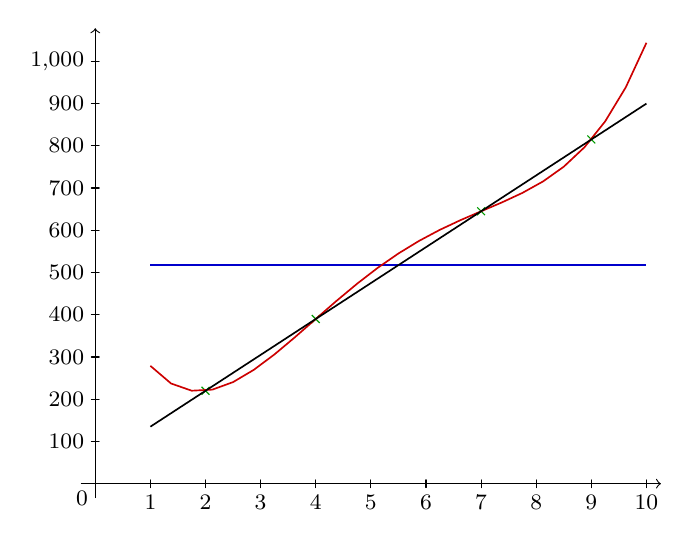
\begin{tikzpicture}[scale=.7]
\datavisualization[school book axes, 
visualize as line=lin,
visualize as line=poly,
visualize as line=mean,
visualize as scatter=data,
y axis={scaling = min at 0cm and max at 8cm,ticks={step=100}},
style sheet=strong colors
] 
data [set=lin,format=function] {
var x : interval [1:10];
func y = 85*(\value x)+50;
}
data [set=poly,format=function] {
var x : interval [1:10];
func y = 554 +(\value x)*(-421+167*(\value x)-22*(\value x)*(\value x)+(\value x)*(\value x)*(\value x));
}
data [set=mean,format=function] {
var x : interval [1:10];
func y = 517.5;
}
data[set=data]  {
x, y
2, (85*2+50)
4, (85*4+50)
7, (85*7+50)
9, (85*9+50)
}
;
\end{tikzpicture}
\end{center}
\end{frame}

\begin{frame}{Znajdźmy więcej prosiaków: zbiór testowy}
Czarne: $y=85x+50 \qquad MSE=0$ \\
Czerwone: $y=x^4-22x^3+167x^2-421x+554 \qquad MSE=7296$ \\
Niebieskie: $y=517{,}5 \qquad MSE=64423$

\begin{center}
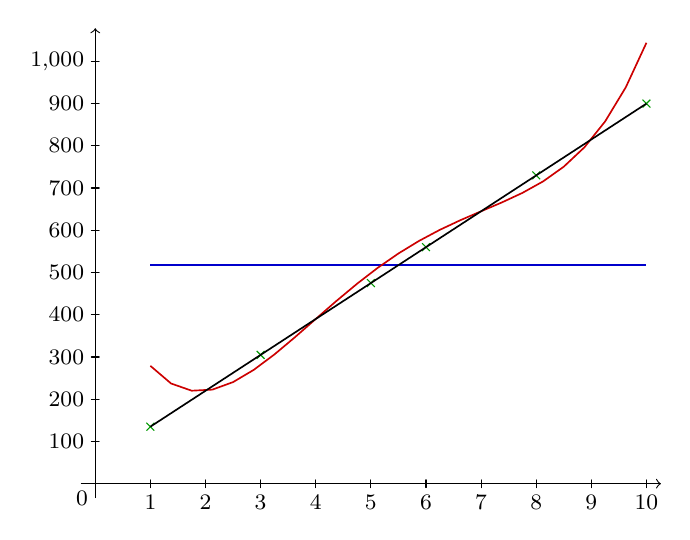
\begin{tikzpicture}[scale=.7]
\datavisualization[school book axes, 
visualize as line=lin,
visualize as line=poly,
visualize as line=mean,
visualize as scatter=data,
y axis={scaling = min at 0cm and max at 8cm,ticks={step=100}},
style sheet=strong colors
] 
data [set=lin,format=function] {
var x : interval [1:10];
func y = 85*(\value x)+50;
}
data [set=poly,format=function] {
var x : interval [1:10];
func y = 554 +(\value x)*(-421+167*(\value x)-22*(\value x)*(\value x)+(\value x)*(\value x)*(\value x));
}
data [set=mean,format=function] {
var x : interval [1:10];
func y = 517.5;
}
data[set=data,format=function]  {
var x : {1,3,5,6,8,10};
func y = 85*(\value x)+50;
}
;
\end{tikzpicture}
\end{center}
\end{frame}

\begin{frame}{Czy prosiaki uczące i prosiaki testowe się różnią?}
\begin{block}{Założenie i.i.d -- Identicially and idependently distributed}
Zakłada się, że wszystkie przykłady uczące i testowe pochodzą \alert{z tego samego rozkładu prawdopodobieństwa}, i zostały wybrane z niego \alert{niezależnie od siebie}.
\end{block}
\end{frame}

\begin{frame}{Zbyt słabe i nadmierne dopasowanie}
\begin{block}{Zbyt słabe dopasowanie \ang{underfitting}}
Duży błąd na zbiorze uczącym i duży błąd na zbiorze testowym
\end{block}
\vfill
\begin{block}{Nadmierne dopasowanie (przeuczenie) \ang{overfitting}}
Mały błąd na zbiorze uczącym i duży błąd na zbiorze testowym
\end{block}
\end{frame}

\begin{frame}{Zbyt słabe i nadmierne dopasowanie}
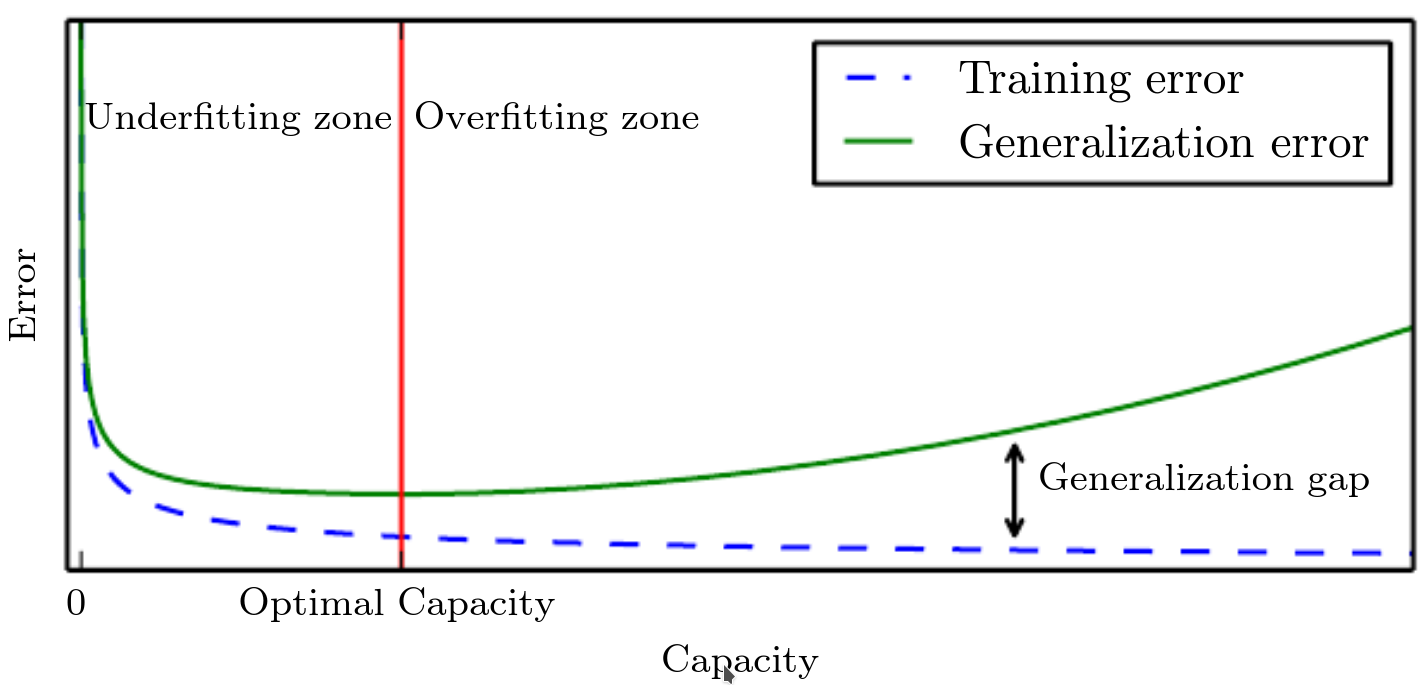
\includegraphics[width=\textwidth]{underfitting-overfitting.png}
\vfill
{\footnotesize I. Goodfellow, Y. Bengio, A. Courville \emph{Deep Learning} MIT Press 2016, str. 112}
\end{frame}

\begin{frame}{Parametry i hiperparametry}
\begin{description}
\item[parametry] są dobierane przez algorytm w procesie uczenia, np. wektor $\vec{w}$ w regresji liniowej
\item[hiperparametry] są dobierane przez użytkownika, żeby sterować procesem uczenia, np. stopień wielomianu w regresji wielomianowej
\end{description}
\end{frame}

\begin{frame}{Dobór hiperparametrów i zbiór walidujący}
\begin{block}{}
Dobór hiperparametrów za pomocą zbioru testowego prowadzi do przeuczenia
\end{block}

\pause
\vfill

\begin{itemize}
\item dobór \alert{parametrów} (uczenie) przez minimalizację błędu na zbiorze \alert{uczącym}
\item dobór \alert{hiperparametrów} przez minimalizację błędu na zbiorze \alert{walidującym}
\item szacowanie jakości na zbiorze \alert{testowym}
\end{itemize}
\end{frame}

\begin{frame}{Zwyczajowy podział danych}

Podział losowy w nastepujących proporcjach
\begin{description}
\item[zbiór testowy] $70\%$
\item[zbiór walidujący] $10\%$
\item[zbiór testowy] $20\%$
\end{description}
\end{frame}

\begin{frame}{Sprawdzian krzyżowy \ang{cross-validation}}
\begin{enumerate}
\item Zbiór uczący dzielony jest na $k$ podzbiorów
\item Dla $i=1,2,\ldots, k$:
\begin{description}
\item[zbiór walidujący] podzbiór $i$
\item[zbiór uczący]  wszystkie pozostałe podzbiory
\end{description}
\item Za wynik walidacji przyjmuje się średnią ze wszystkich $k$ walidacji (odchylenie standardowe gratis!)
\end{enumerate}

\vfill
Jakie są zalety i wady w stosunku do poprzedniego podejścia?
\end{frame}

\begin{frame}{Problemy z regresją liniową}
\[ \vec{w}={\underbrace{\left(\vec{X}^T\vec{X}\right)}_{p\times p}}^{-1}\vec{X}^T\vec{y} \]
\begin{itemize}
\item<+-> Złożoność odwracania macierzy: $O(p^{2.4})$ \\
\item<+-> Problemy numeryczne
\item<+-> Trudności z uogólnieniem: trzeba \alert{rozwiązać} równanie
\end{itemize}
\end{frame}

\begin{frame}{Schodzenie po gradiencie \ang{gradient descent}}
\centering
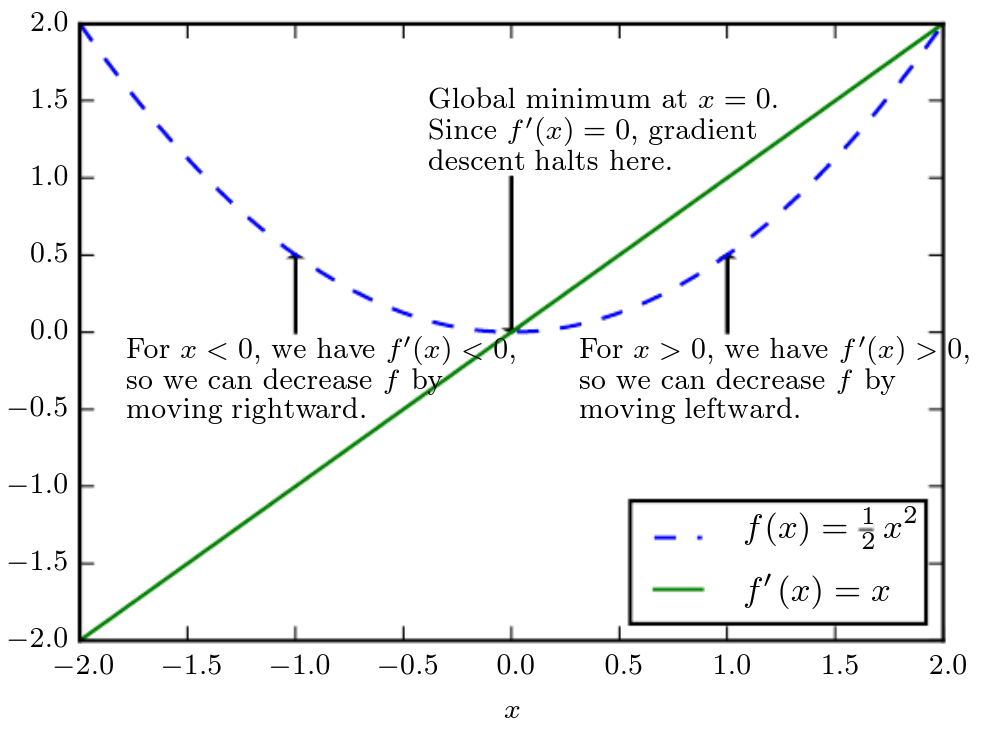
\includegraphics[width=.87\textwidth]{grad.png}
{\vfill\footnotesize I. Goodfellow, Y. Bengio, A. Courville \emph{Deep Learning} MIT Press 2016, str. 80}
\end{frame}

\begin{frame}{Schodzenie po gradiencie \ang{gradient descent}}
\centering
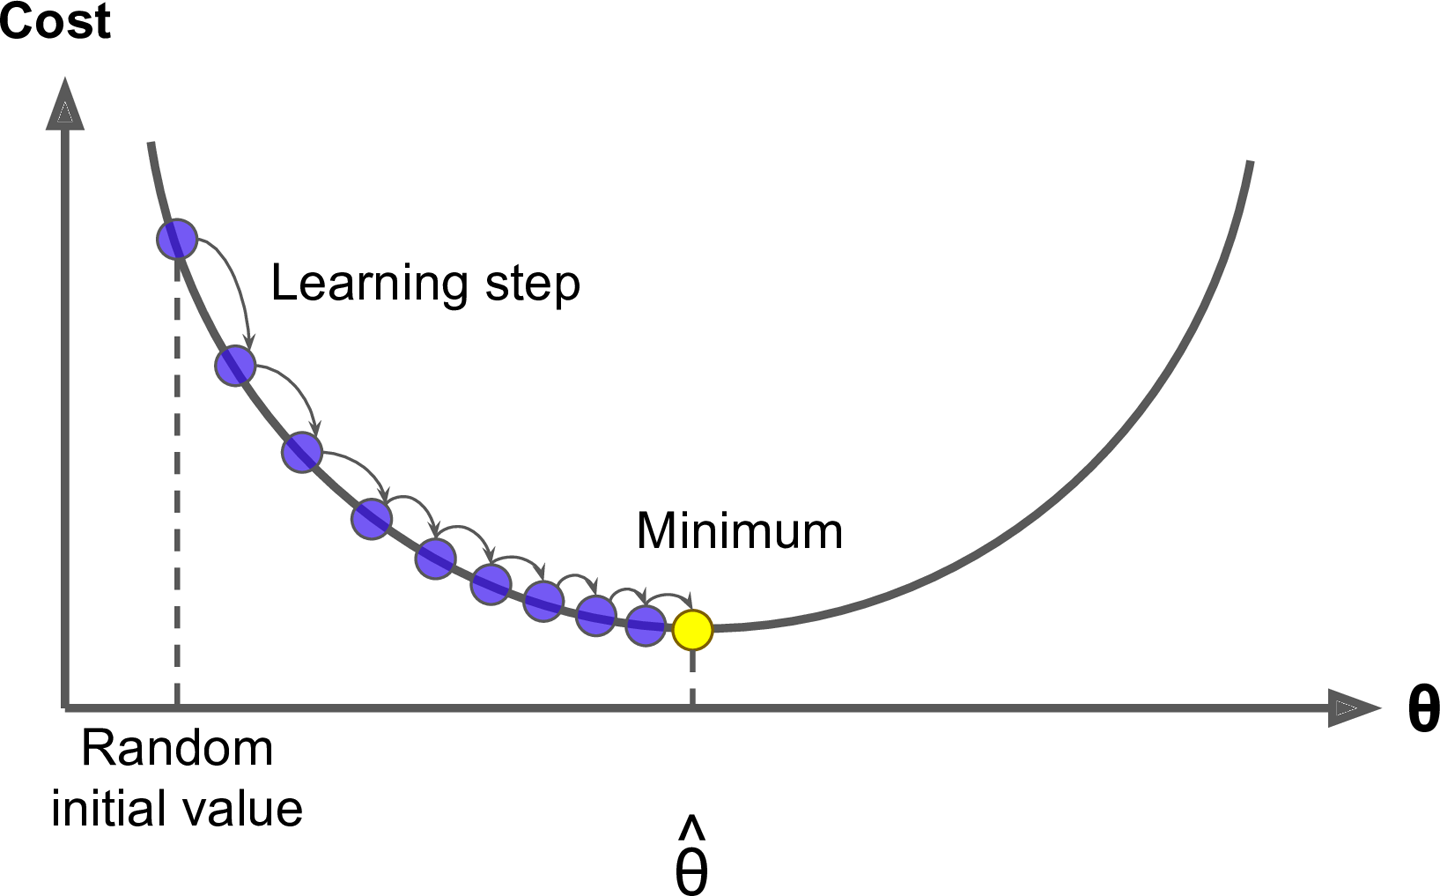
\includegraphics[width=.95\textwidth]{grad2.png}
{\vfill\footnotesize A. Géron, \emph{Hands-On Machine Learning with Scikit-Learn and TensorFlow} 2017, str. 111}
\end{frame}

\begin{frame}{Schodzenie po gradiencie \ang{gradient descent}}
\[ J(w, b) = \frac{1}{n}\sum_{i=1}^n \left(wx_i+b-y_i\right)^2 \]
\[ \grad J(w,b) = \begin{bmatrix}
\frac{1}{n}\sum_{i=1}^n 2x_i\left(wx_i+b-y_i\right) \\
\frac{1}{n}\sum_{i=1}^n 2\left(wx_i+b-y_i\right)
\end{bmatrix}
=
\frac{2}{n}\sum_{i=1}^n 
\left(wx_i+b-y_i\right) \begin{bmatrix}
x_i \\
1
\end{bmatrix}
\]
\[
\begin{bmatrix}
w' \\ b'
\end{bmatrix}
=
\begin{bmatrix}
w \\ b
\end{bmatrix}
-\varepsilon \grad J(w,b)
\]
\end{frame}

\begin{frame}{Prosiaki schodzące po gradiencie}
\begin{center}
\begin{tabular}{rrrrrr}
krok & $w$ & $b$ & $MSE$ & $\grad_w MSE$ & $\grad_b MSE$ \\
\hline
0 & 0 & 0 & $1280750$ & $-27700$ & $-1035$ \\
1 & $166.20$ & $6.21$ & $840233$ & $22433$ & $805$ \\
2 & $31.60$ & $1.38$ & $551427$ & $-18159$ & $-684$ \\
3 & $140.56$ & $5.48$ & $362082$ & $14708$ & $522$ \\
\ldots \\
$3102$ & $85.01$ & $49.96$ & $0.001$ & $0.002$ & $-0.014$ \\
\ldots \\
$6590$ & $85.00$ & $50.00$ & $0.000$ & $0.000$ & $0.000$ \\
\end{tabular}
\end{center}
\end{frame}


\begin{frame}{Prosiaki schodzące po gradiencie}
\begin{center}
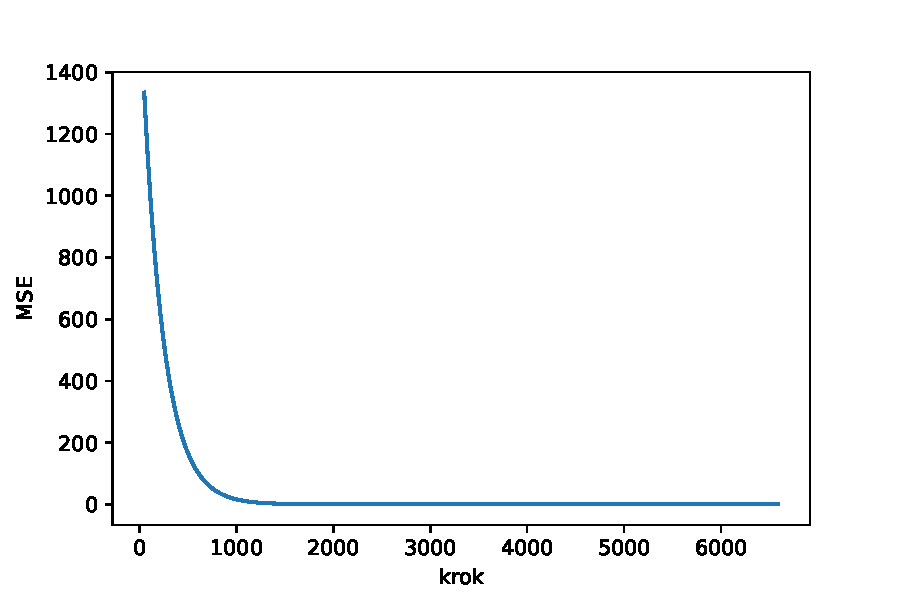
\includegraphics[width=.9\textwidth]{grad-prosiaki.pdf}
\end{center}

Warunek stopu: $MSE<1^{-10}$ lub $\grad J<1^{-10}$
\end{frame}

\begin{frame}{Stochastyczne schodzenie po gradiencie}
\begin{block}{\emph{Stochastic gradient descent}}
Jeżeli przykładów jest dużo, to schodzenie po gradiencie może być powolne.
Zamiast tego w każdym kroku wybieramy losowo \alert{jeden} przykład uczący i obliczamy gradient wyłącznie na jego podstawie.
\end{block}
\end{frame}

\begin{frame}{Stochastyczne schodzenie po gradiencie}
\centering
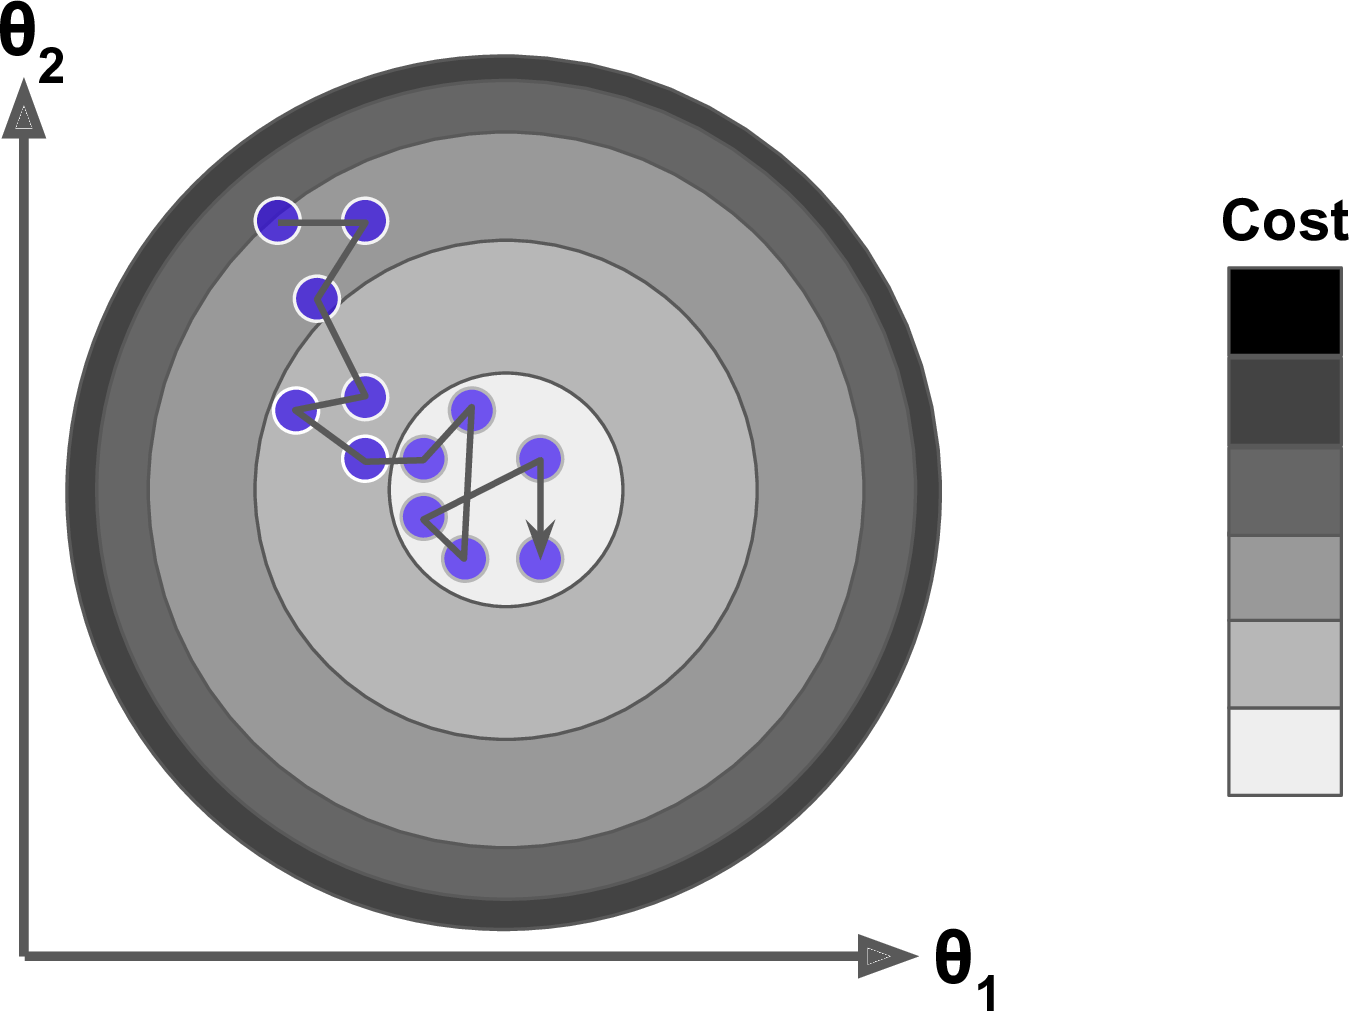
\includegraphics[width=.7\textwidth]{sgd.png}
{\vfill\footnotesize A. Géron, \emph{Hands-On Machine Learning with Scikit-Learn and TensorFlow} 2017, str. 117}
\end{frame}

\begin{frame}{Prosiaki stochastycznie schodzące po gradiencie}
\begin{center}
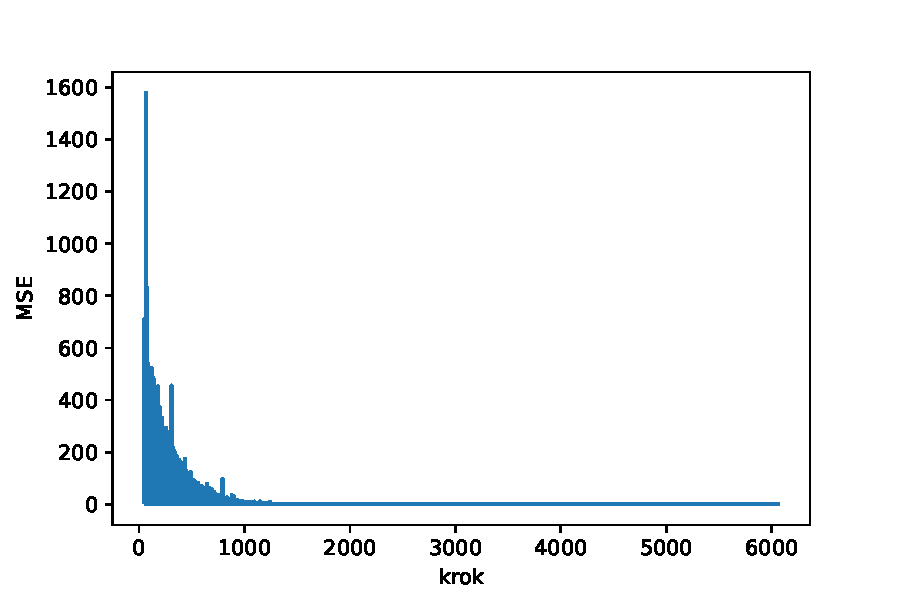
\includegraphics[width=.9\textwidth]{sgd-prosiaki.pdf}
\end{center}

Warunek stopu: $MSE$ przez ostatnie 10 kroków $<1^{-10}$
\end{frame}

\begin{frame}{Schodzenie po gradiencie z mini-grupami}
\begin{block}{\emph{Mini-batch gradient descent}}
W kolejnych krokach schodzenia po gradiencie wybieramy (niewielki) podzbiór przykładów uczących do obliczeń
\end{block}
\begin{itemize}
\item stabilniejszy
\item zysk wydajnościowy z obliczeń macierzowych
\end{itemize}
\end{frame}


\begin{frame}{Problemy ze schodzeniem po gradiencie}
\centering
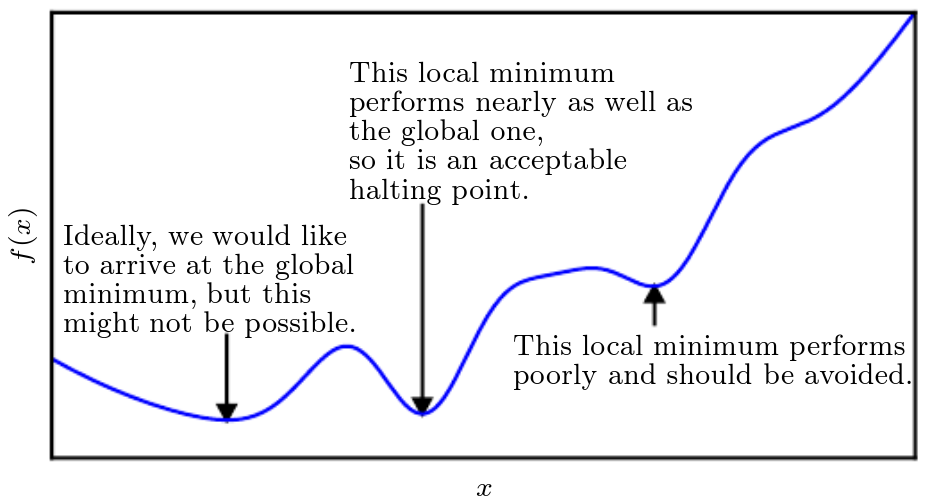
\includegraphics[width=\textwidth]{grad-problemy.png}
{\vfill\footnotesize I. Goodfellow, Y. Bengio, A. Courville \emph{Deep Learning} MIT Press 2016, str. 81}
\end{frame}

\begin{frame}{Problemy ze schodzeniem po gradiencie}
\centering
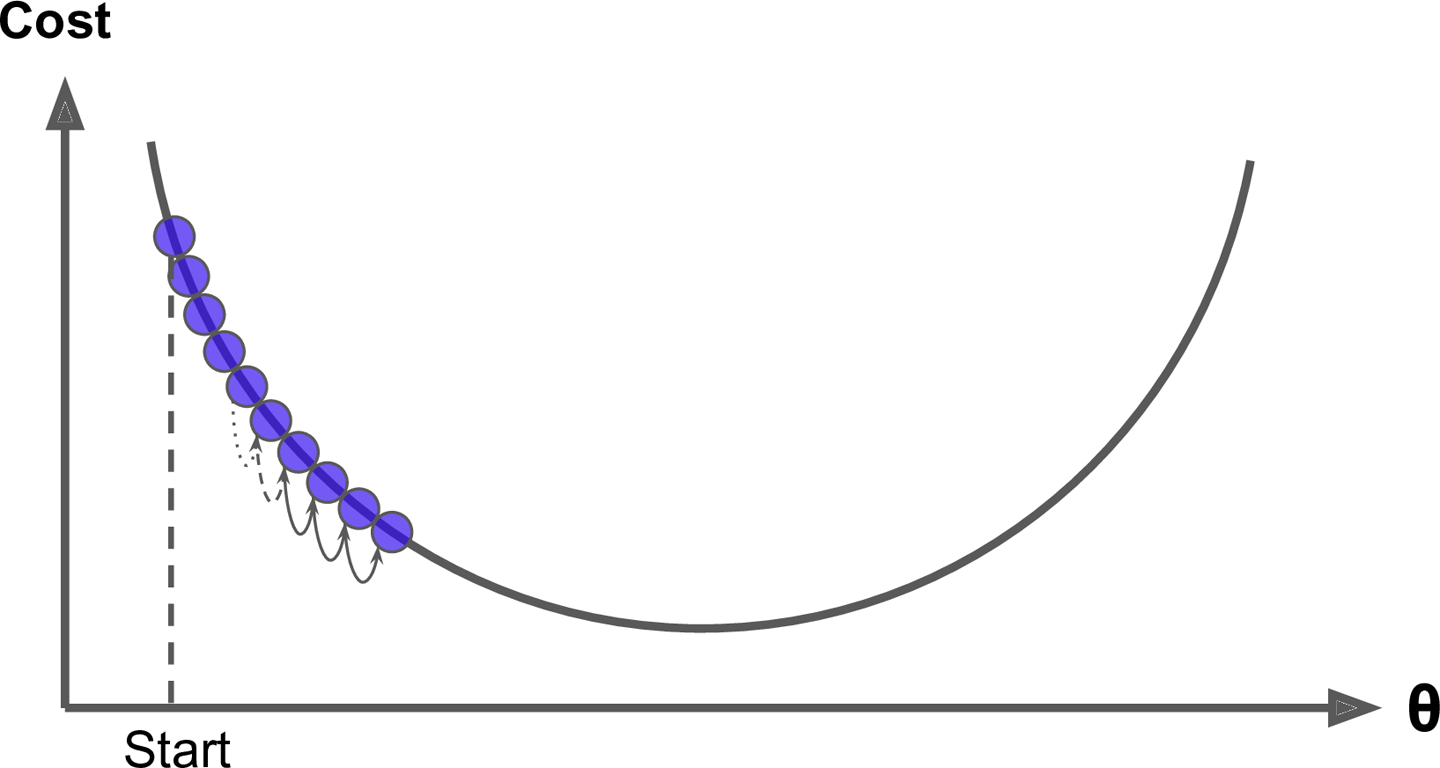
\includegraphics[width=.95\textwidth]{grad-e-toosmall.png}
{\vfill\footnotesize A. Géron, \emph{Hands-On Machine Learning with Scikit-Learn and TensorFlow} 2017, str. 112}
\end{frame}

\begin{frame}{Problemy ze schodzeniem po gradiencie}
\centering
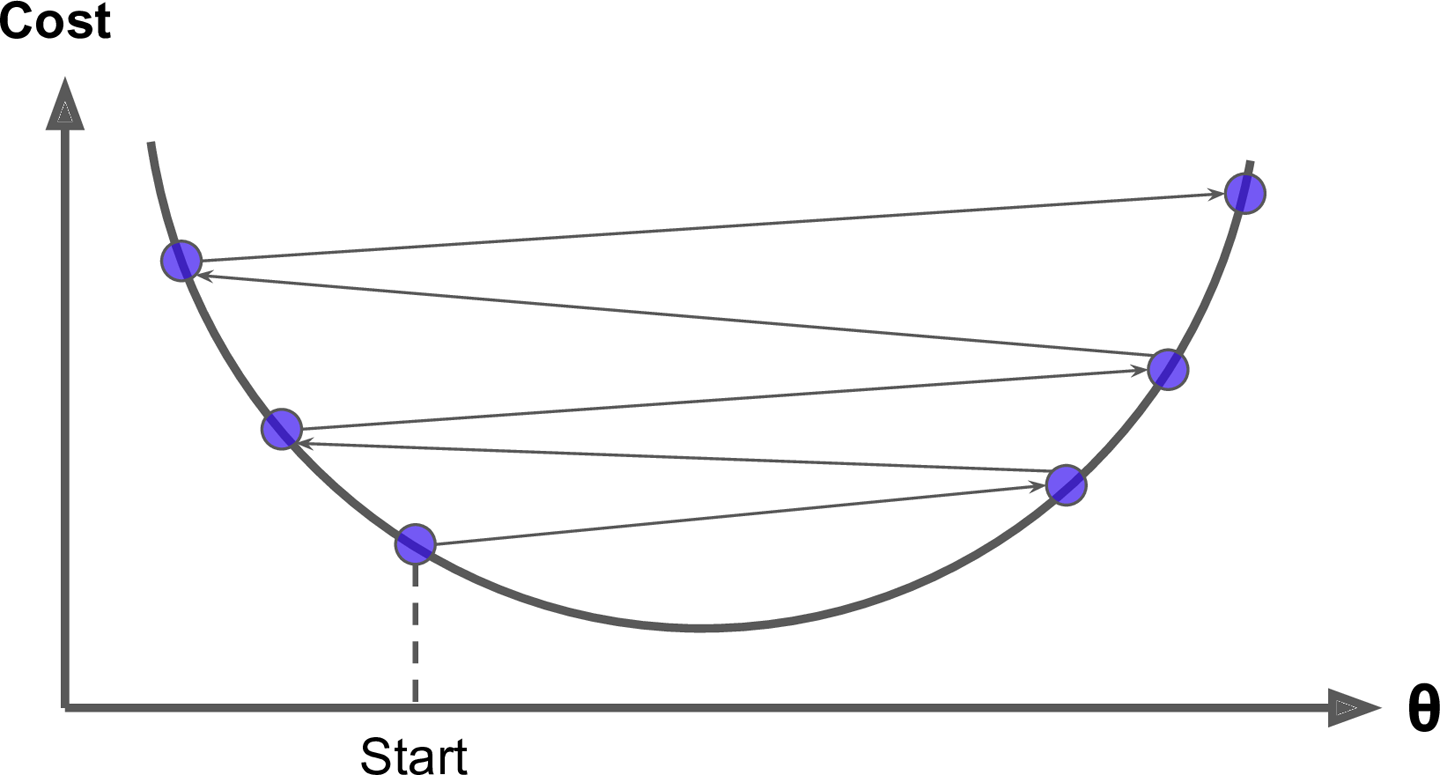
\includegraphics[width=.95\textwidth]{grad-e-toolarge.png}
{\vfill\footnotesize A. Géron, \emph{Hands-On Machine Learning with Scikit-Learn and TensorFlow} 2017, str. 112}
\end{frame}

\begin{frame}{Problemy ze schodzeniem po gradiencie}
\centering
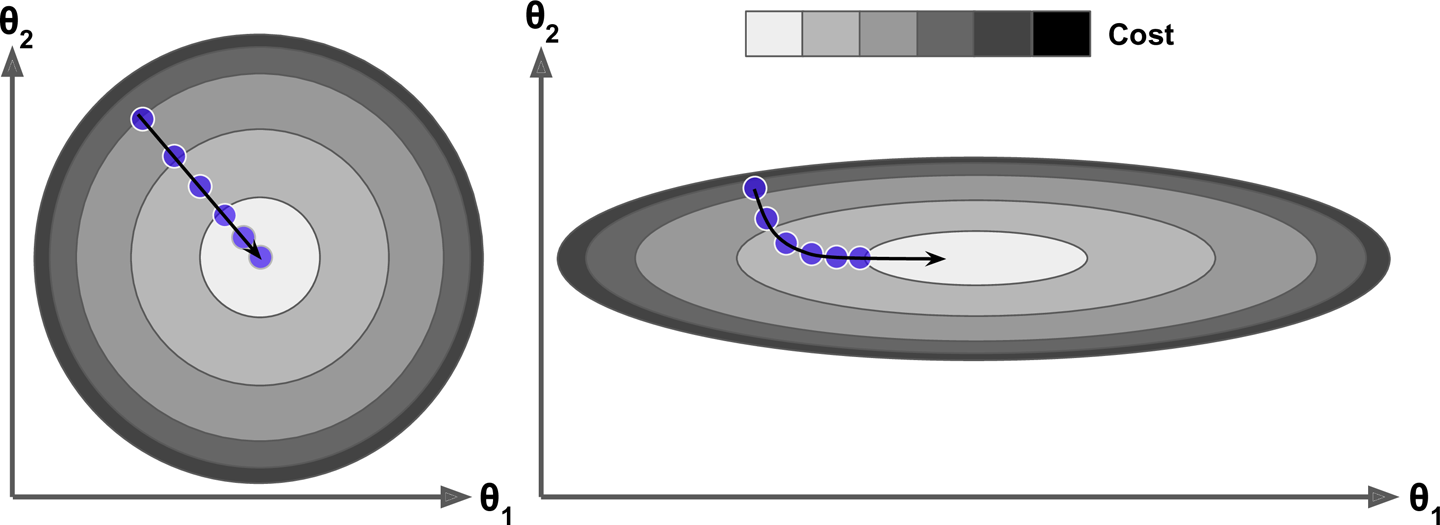
\includegraphics[width=.95\textwidth]{grad-nofscaling.png}
{\vfill\footnotesize A. Géron, \emph{Hands-On Machine Learning with Scikit-Learn and TensorFlow} 2017, str. 113}
\end{frame}

\begin{frame}{Skalowanie}
\begin{description}
\item[standaryzacja] \[ X_{i,j} = \frac{X_{i,j}-\overline{X_{\cdot,j}}}{\sigma_{X_{\cdot,j}}} \]
\item[min-max] \[ X_{i,j} = \frac{X_{i,j}-\min_k\{X_{k,j}\}}{\max_k\{X_{k,j}\}-\min_k\{X_{k,j}\}} \]
\end{description}

\vfill
\alert{Czym różnią się te dwa podejścia?}
\end{frame}

\begin{frame}{Trochę bardziej skomplikowany problem regresji}
\[ y=0{,}02x^3+10x+5+N(0,100) \]
niebieski: proces, pomarańczowy: zb. treningowy, zielony: zb. walidujący
\centering
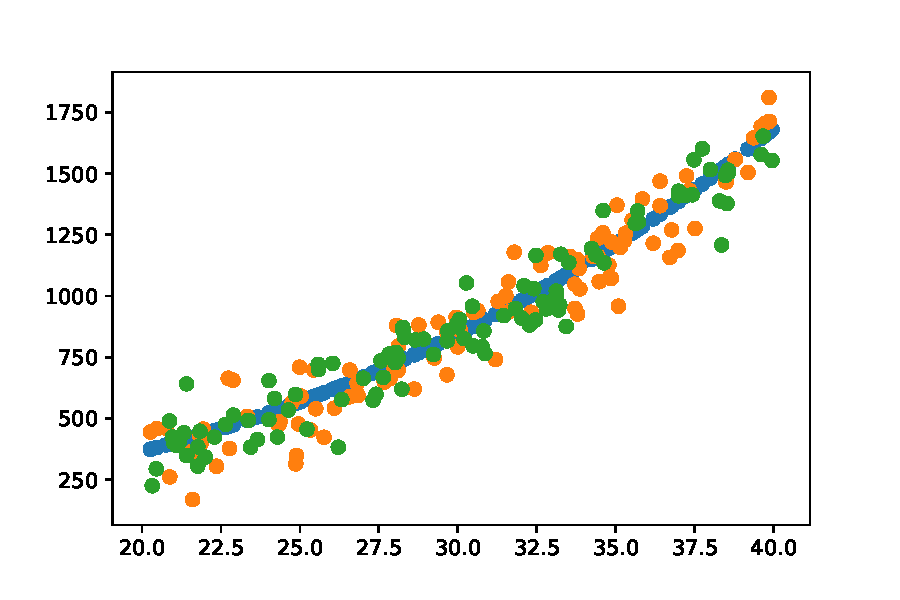
\includegraphics[width=.9\textwidth]{reg-2deg-with-noise.pdf}
\end{frame}

\begin{frame}{Możliwe rozwiązanie (I)}
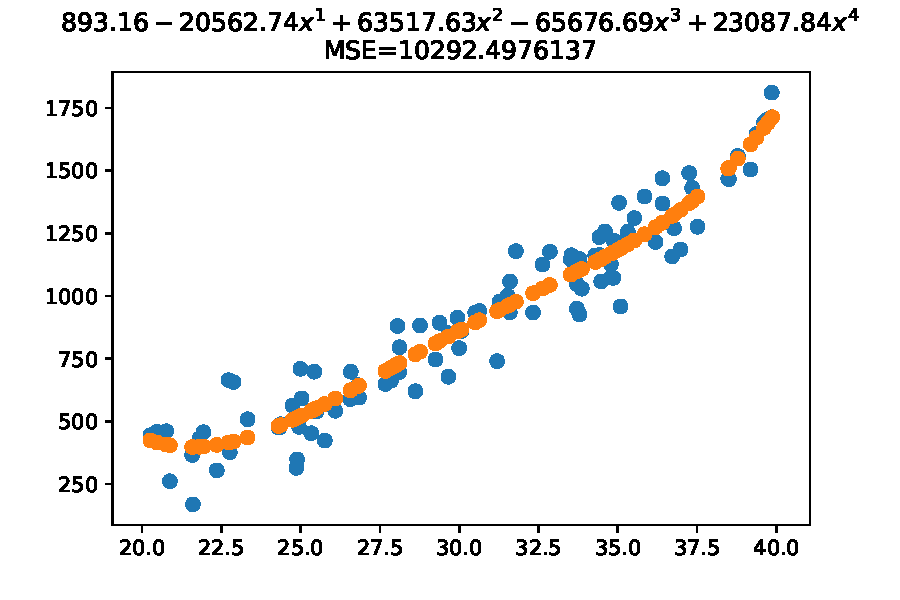
\includegraphics[width=\textwidth]{reg-2deg-with-noise-ridge0.pdf}
\end{frame}

\begin{frame}{Możliwe rozwiązanie (II)}
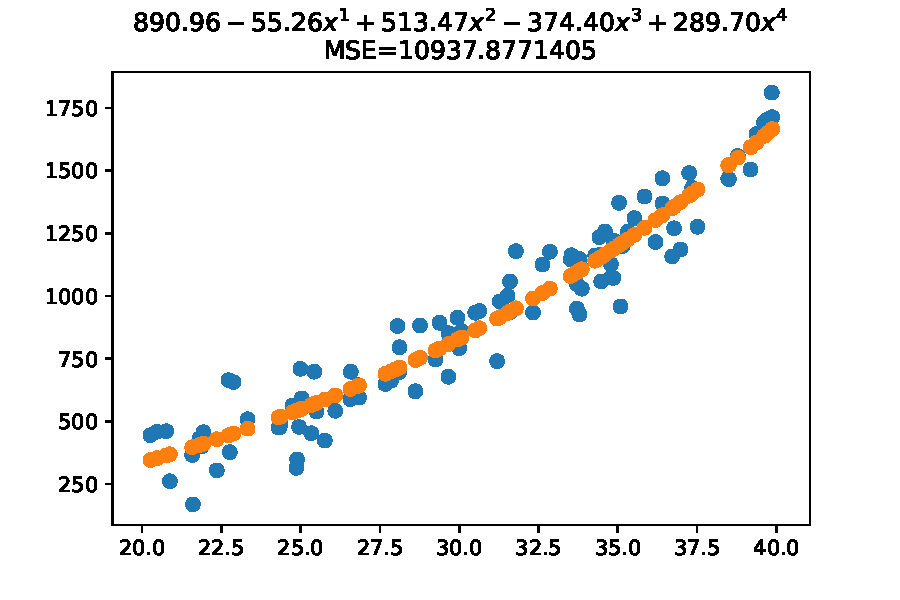
\includegraphics[width=\textwidth]{reg-2deg-with-noise-ridge0_001.pdf}
\end{frame}

\begin{frame}{Możliwe rozwiązanie (III)}
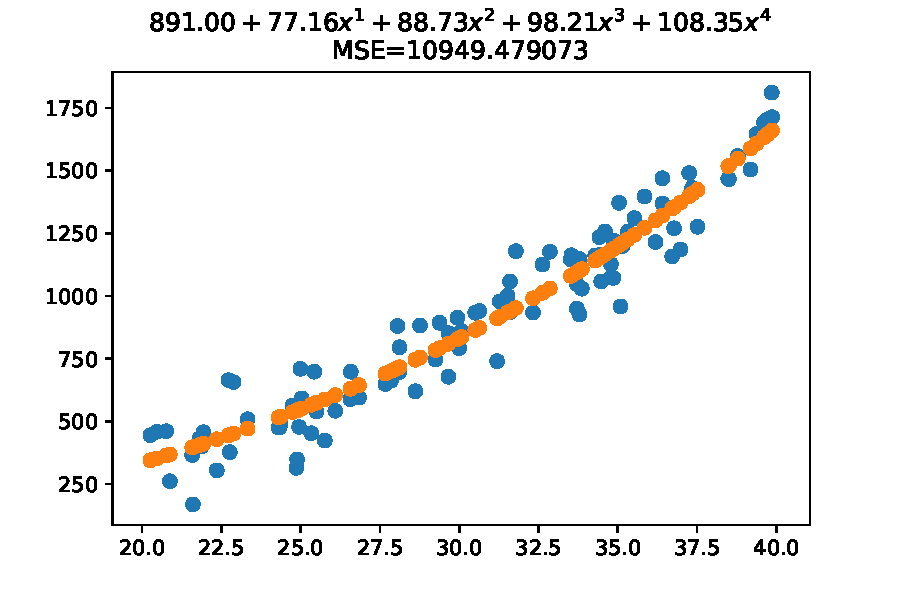
\includegraphics[width=\textwidth]{reg-2deg-with-noise-ridge1.pdf}
\end{frame}

\begin{frame}{Możliwe rozwiązanie (IV)}
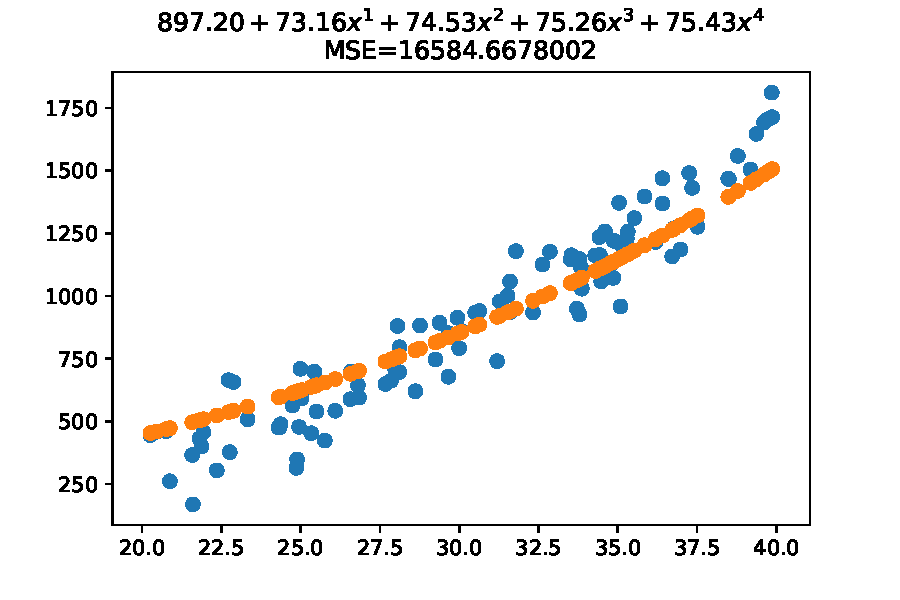
\includegraphics[width=\textwidth]{reg-2deg-with-noise-ridge100.pdf}
\end{frame}

\begin{frame}{Możliwe rozwiązanie (V)}
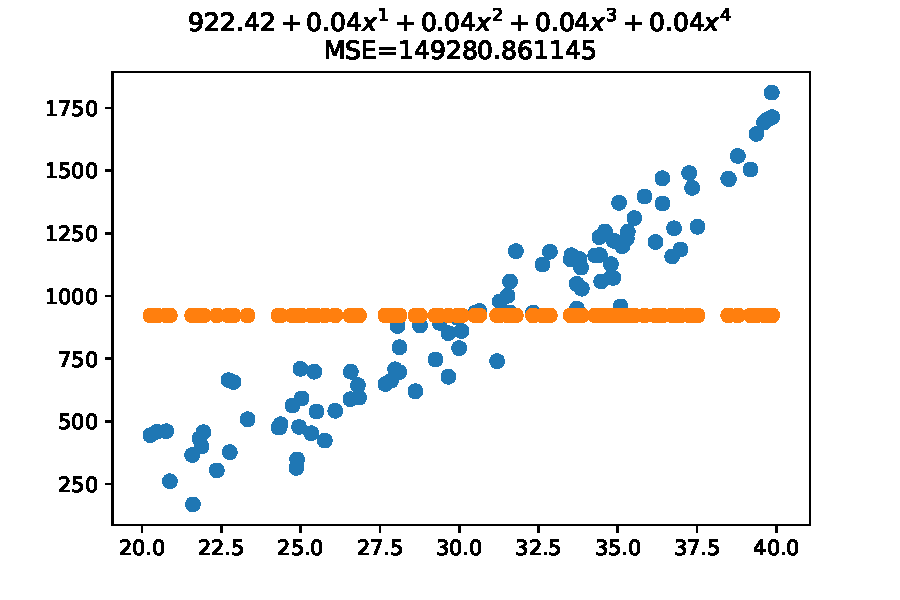
\includegraphics[width=\textwidth]{reg-2deg-with-noise-ridge1000000.pdf}
\end{frame}

\begin{frame}{Regularyzacja Ridge}
\[ J(\vec{w}) = MSE(\vec{w}) + \alpha \underbrace{\frac{1}{2}\sum_{\alert{i=1}}^n w_i^2}_{kara} \]
\end{frame}

\begin{frame}{Porównanie rozwiązań}
\centering
\begin{tabular}{rrrrrr}
$\alpha$ & $MSE_{tr}$  & kara  & całkowity koszt & $MSE_{walid}$ \\
\hline
$0$ & $10292$ & $4651895996$ & $10292$ & $9627$\\
$0.001$ & $10937$ & $245404$ & $11183$ & $8726$\\
$1$ & $10949$ & $17605$ & $28554$ & $8678$\\
$100$ & $16584$ & $11130$ & $1129591$ & $12312$\\
$1000000$ & $149280$ & $0$ & $152023$ & $138743$\\
\end{tabular}

\pause
\vfill
\alert{Ile współczynników miały rozważane wielomiany?}
\end{frame}

\begin{frame}{Możliwe rozwiązanie (I)}
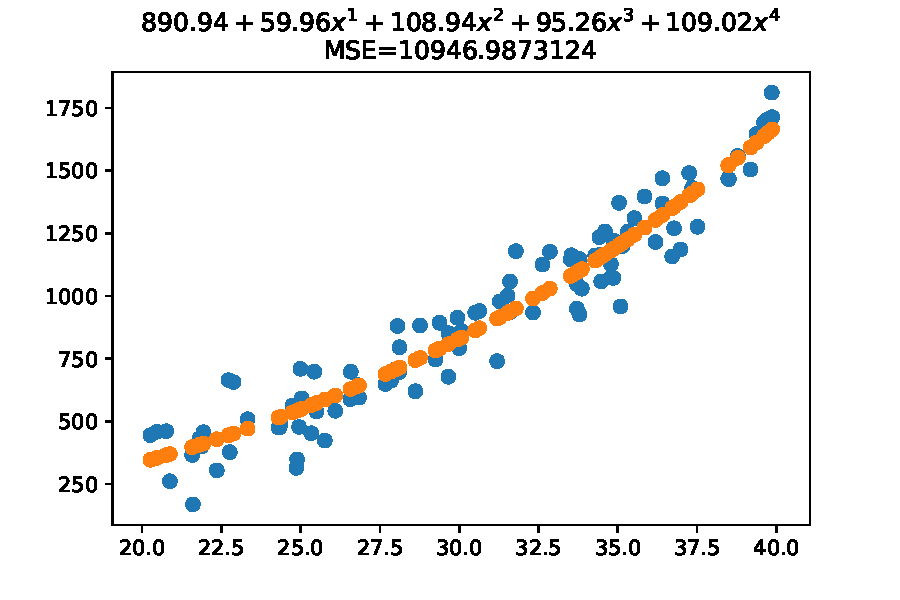
\includegraphics[width=\textwidth]{reg-3deg-with-noise-lasso0.pdf}
\end{frame}
\begin{frame}{Możliwe rozwiązanie (II)}
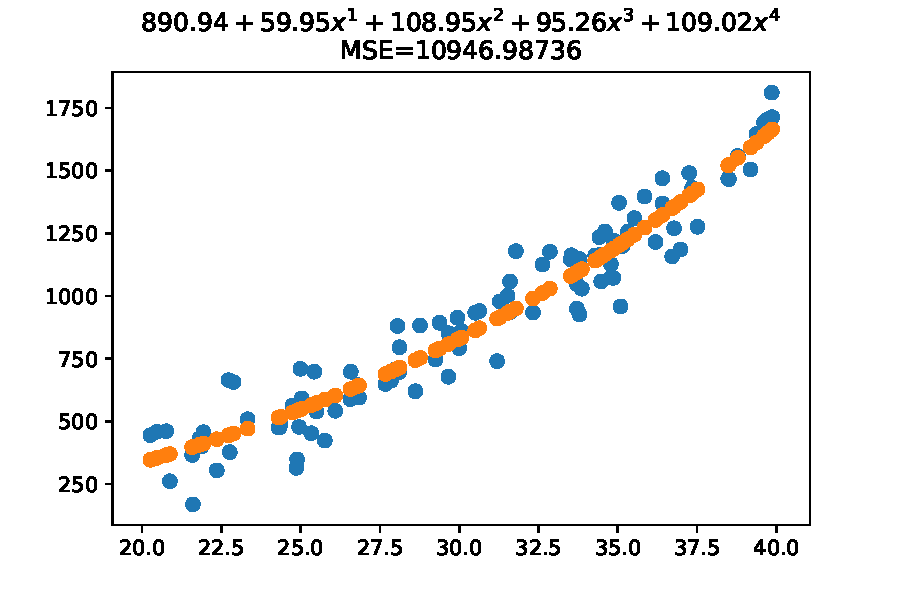
\includegraphics[width=\textwidth]{reg-3deg-with-noise-lasso0_001.pdf}
\end{frame}
\begin{frame}{Możliwe rozwiązanie (III)}
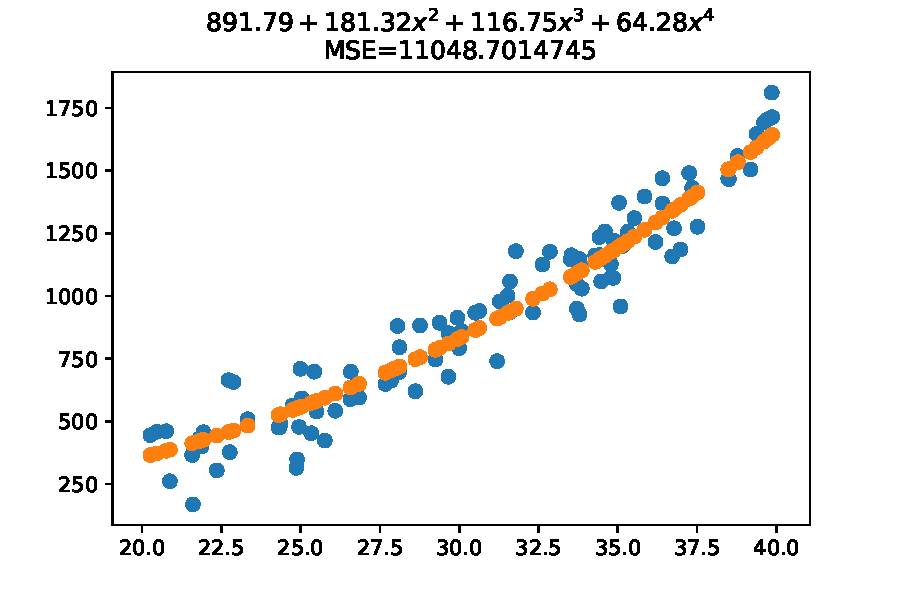
\includegraphics[width=\textwidth]{reg-3deg-with-noise-lasso10.pdf}
\end{frame}
\begin{frame}{Możliwe rozwiązanie (IV)}
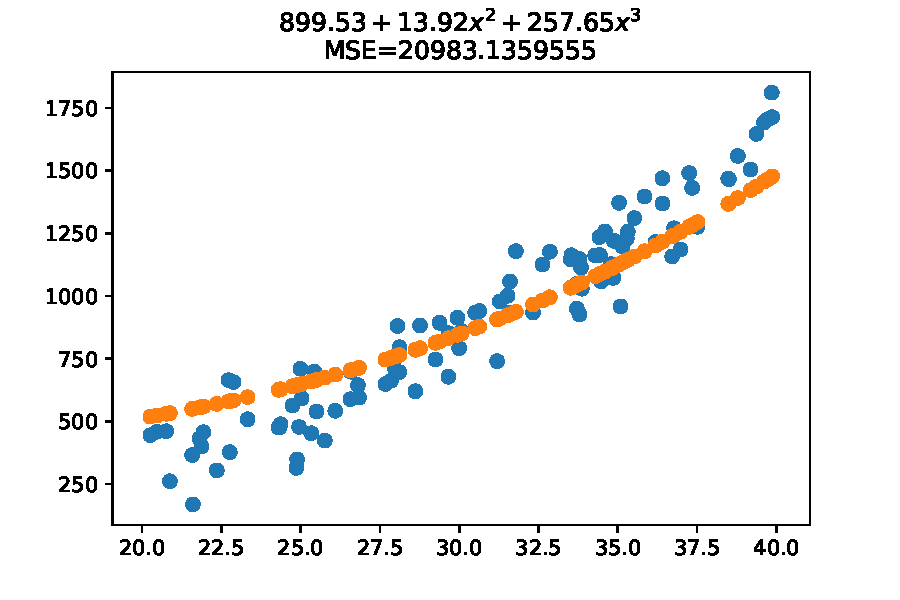
\includegraphics[width=\textwidth]{reg-3deg-with-noise-lasso100.pdf}
\end{frame}
\begin{frame}{Możliwe rozwiązanie (V)}
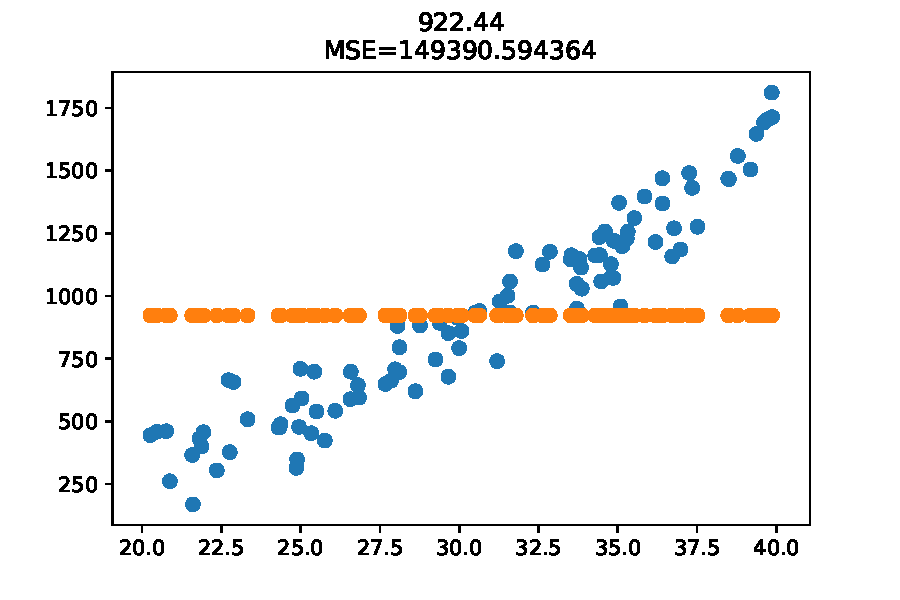
\includegraphics[width=\textwidth]{reg-3deg-with-noise-lasso1000000.pdf}
\end{frame}

\begin{frame}{Regularyzacja Lasso}
\[ J(\vec{w}) = MSE(\vec{w}) + \alpha \underbrace{\sum_{\alert{i=1}}^n \left|w_i\right|}_{kara} \]
\end{frame}

\begin{frame}{Porównanie rozwiązań}
\centering
\begin{tabular}{rrrrrrr}
$\alpha$ & \# wsp. & $MSE_{tr}$  & kara  & całkowity koszt & $MSE_{walid}$ \\
\hline
$0$ & $4$ & $10946$ & $18211$ & $10946$ & $8722$\\
$0.001$ & $4$ & $10946$ & $18211$ & $10965$ & $8721$\\
$10$ & $3$ & $11048$ & $25319$ & $264241$ & $8562$\\
$100$ & $2$ & $20983$ & $33287$ & $3349752$ & $16524$\\
$1000000$ & $0$ & $149390$ & $0$ & $149390$ & $138850$\\
\end{tabular}
\end{frame}

\begin{frame}{Dlaczego Lasso się tak zachowuje?}
Obliczmy karę w Ridge i w Lasso dla następujących przypadków:
\begin{enumerate}
\item \[ \vec{w}_1=\begin{bmatrix} 1 \\ 0.05 \end{bmatrix} \]
\pause
\item \[ \vec{w}_2=\vec{w}_1-\begin{bmatrix} 0.01 \\ 0 \end{bmatrix} \]
\pause
\item \[ \vec{w}_3=\vec{w}_1-\begin{bmatrix} 0 \\ 0.01 \end{bmatrix} \]
\end{enumerate}
\pause
\alert{Który przypadek jest lepszy dla regresji Ridge, a który dla Lasso?}
\end{frame}

\begin{frame}{Regularyzacja w GD: wczesne zatrzymanie}
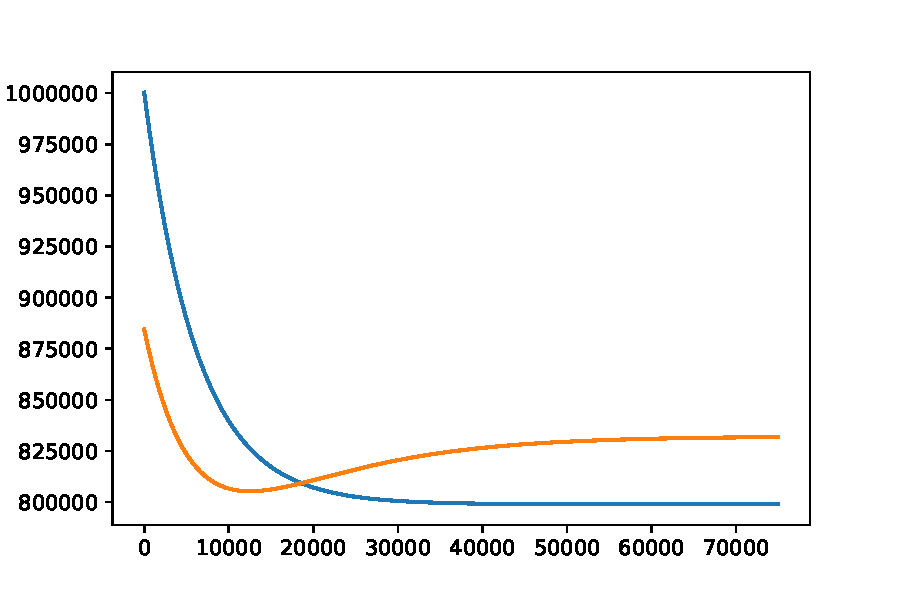
\includegraphics[width=\textwidth]{earlystopping.pdf}
\end{frame}

\begin{frame}{Klasyfikacja}
\begin{block}{Zadanie klasyfikacji binarnej}
Dla danego wektora cech $\vec{x}$ opisującego obiekt przewidzieć czy obiekt należy do klasy \emph{pozytywnej} $y=1$ czy \emph{negatywnej} $y=0$ (lub $y=-1$).
\end{block}
\end{frame}

\begin{frame}{Irysy}
Pomarańczowy: Iris Virginica, niebieski: pozostałe
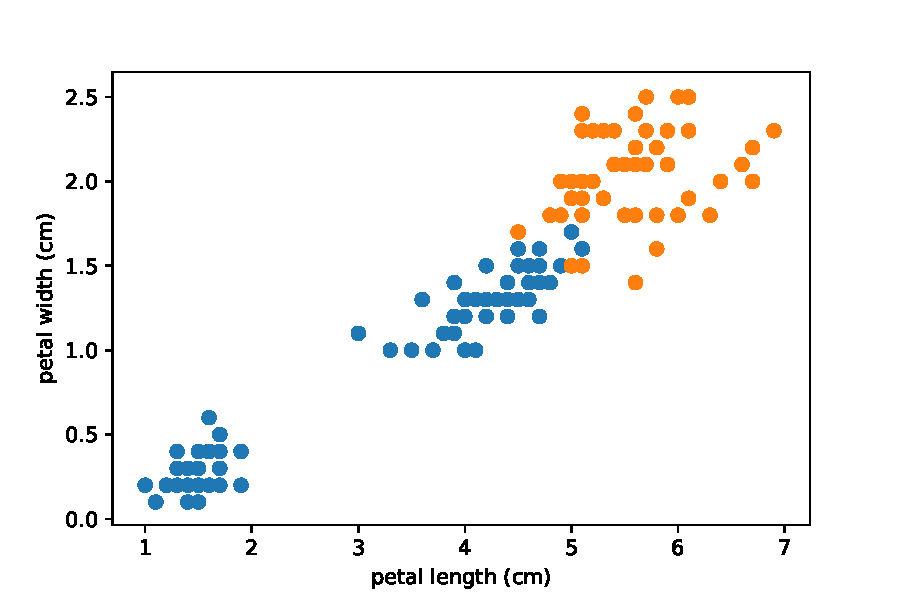
\includegraphics[width=\textwidth]{iris-simplified.pdf}
\end{frame}

\begin{frame}{Przewidywanie prawdopodobieństwa -- regresja liniowa}
Punkty w tle: prawd. Iris Virginica (jaśniej=wyższe)
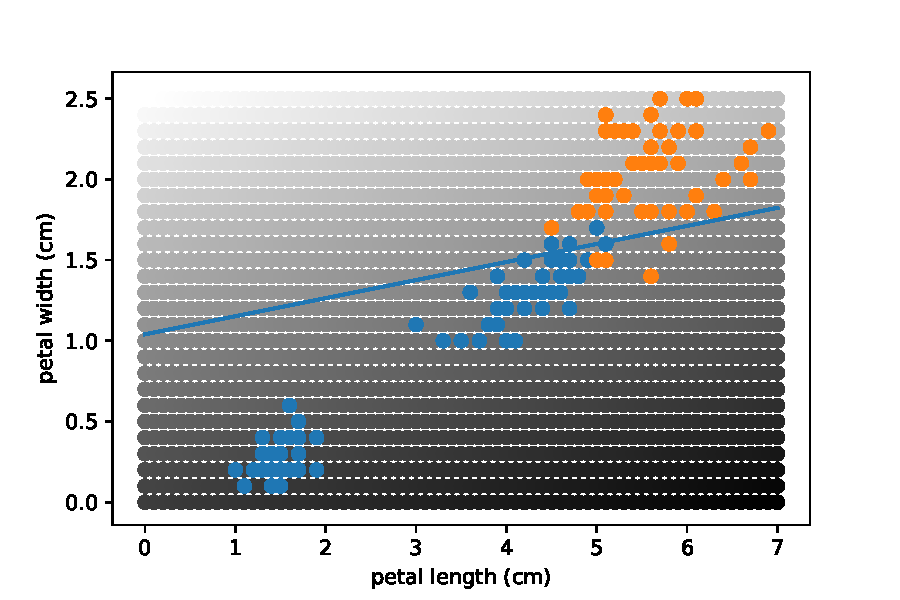
\includegraphics[width=\textwidth]{iris-simplified-linreg.pdf}
\end{frame}

\begin{frame}{Przewidywanie prawdopodobieństwa -- regresja logistyczna}
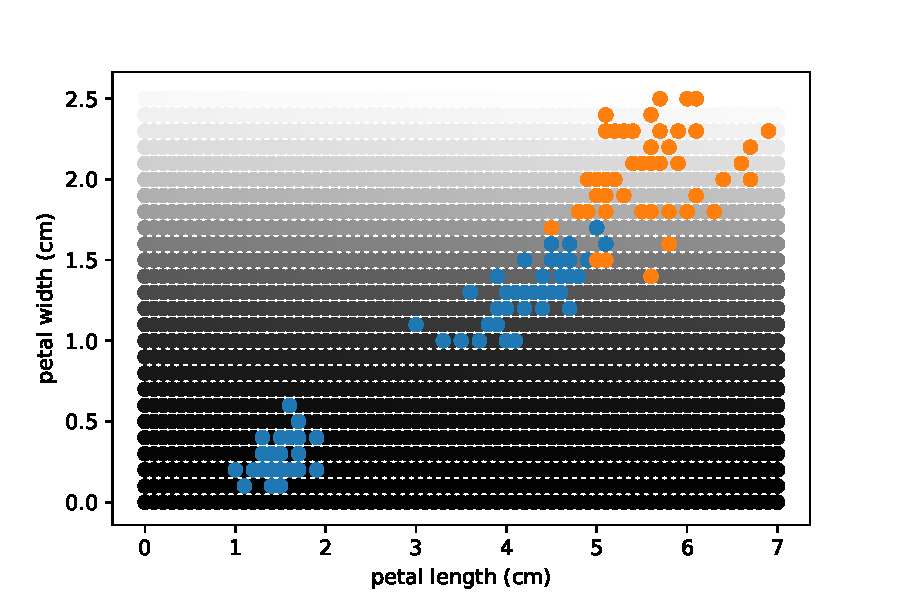
\includegraphics[width=\textwidth]{iris-simplified-logreg.pdf}
\end{frame}

\begin{frame}{Granica decyzyjna (ang. decision boundary)}
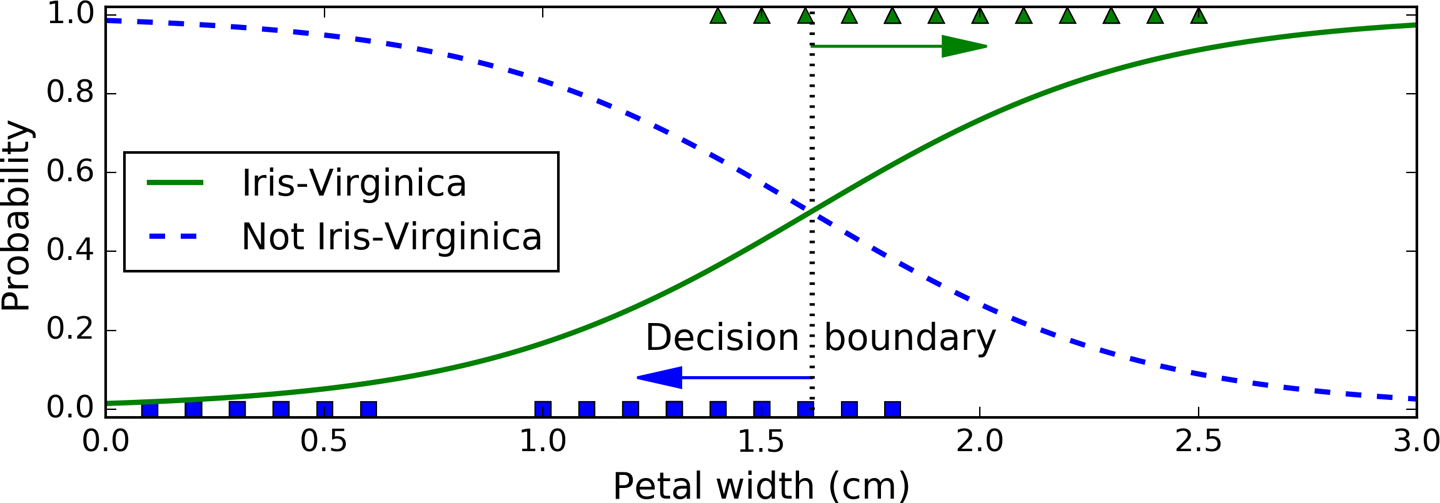
\includegraphics[width=\textwidth]{iris-1attr-decboundary.png}
{\vfill\footnotesize A. Géron, \emph{Hands-On Machine Learning with Scikit-Learn and TensorFlow} 2017}
\end{frame}

\begin{frame}{Granica decyzyjna (ang. decision boundary)}
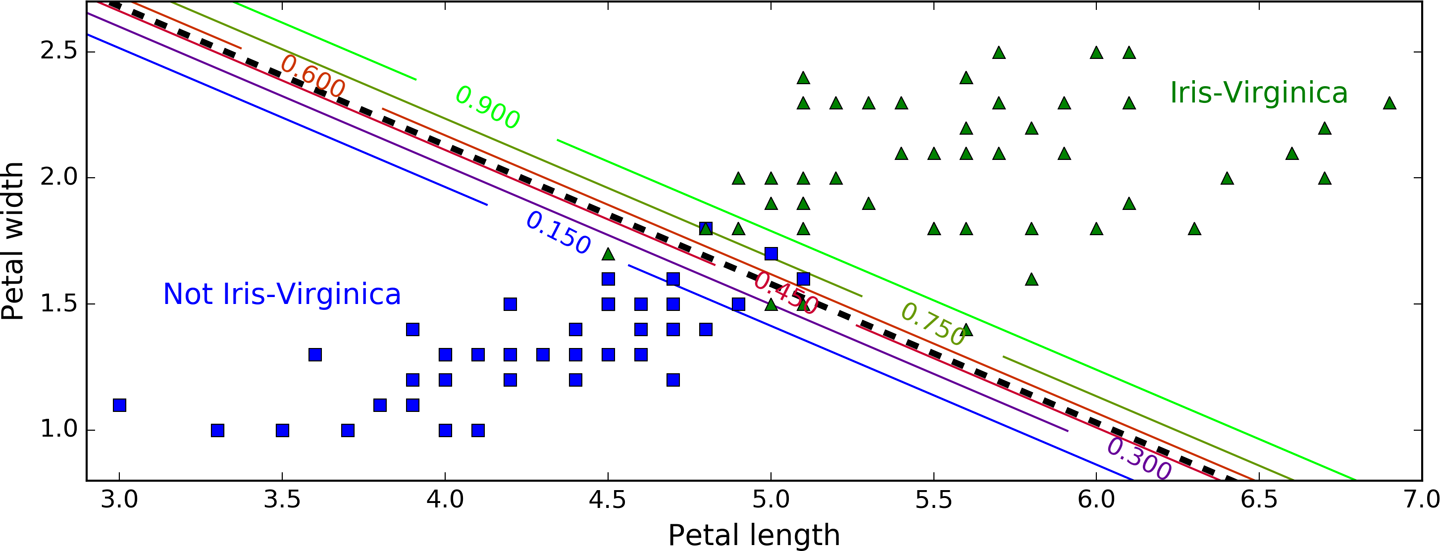
\includegraphics[width=\textwidth]{iris-2attr-decboundary.png}
{\vfill\footnotesize A. Géron, \emph{Hands-On Machine Learning with Scikit-Learn and TensorFlow} 2017}
\end{frame}

\begin{frame}{Funkcja logistyczna}
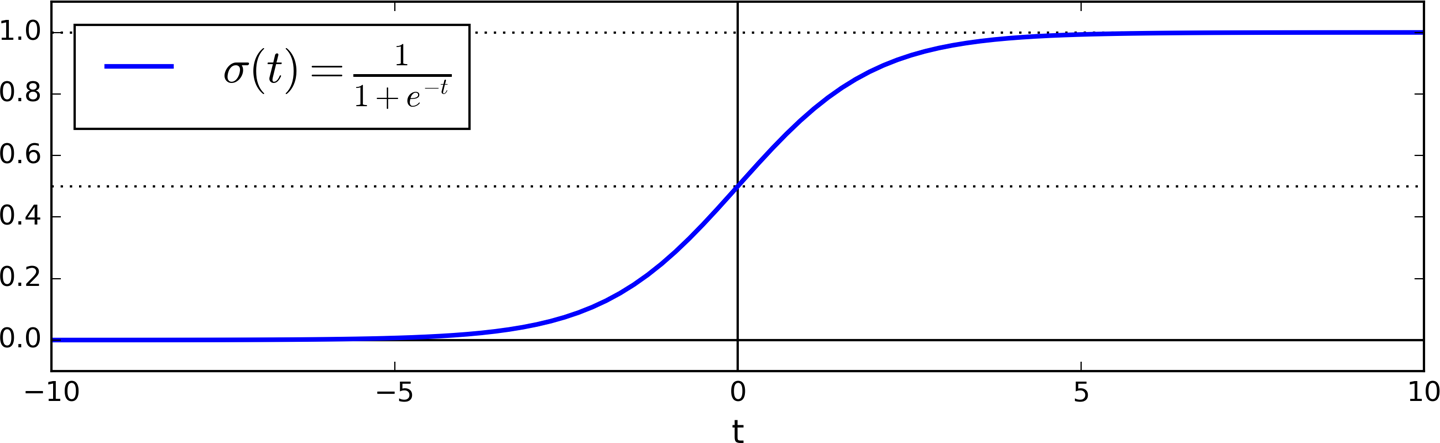
\includegraphics[width=\textwidth]{logistic-function.png}

{\vfill\footnotesize A. Géron, \emph{Hands-On Machine Learning with Scikit-Learn and TensorFlow} 2017}
\end{frame}

\begin{frame}{Pochodna funkcji logisytcznej}
\[ \sigma(t) = \frac{1}{1+e^{-t}} \]

\begin{block}{Zadanie}
Wiadomo, że $\sigma(t_0)=.1$. Czy da się na tej podstawie prosto obliczyć wartość pochodnej $\sigma'(t)$ w punkcie $t_0$?
\end{block}

\note{
\begin{gather*}
\sigma'(t)=-\left(\frac{1}{1+e^{-t}}\right)^2\cdot(-e^{-t})=\ldots=\sigma(t)(1-\sigma(t))
\end{gather*}
}
\end{frame}

\begin{frame}{Regresja logistyczna}
\begin{gather*}
\hat{p} = \sigma(\vec{x}\vec{w}) \\
\hat{y} = \begin{cases}
1 & \hat{p} \geq 0{,}5 \\
0 &\hat{p} < 0{,}5 \\
\end{cases}
\end{gather*}
\end{frame}

\begin{frame}{Funkcja kosztu dla pojedynczego przykładu}
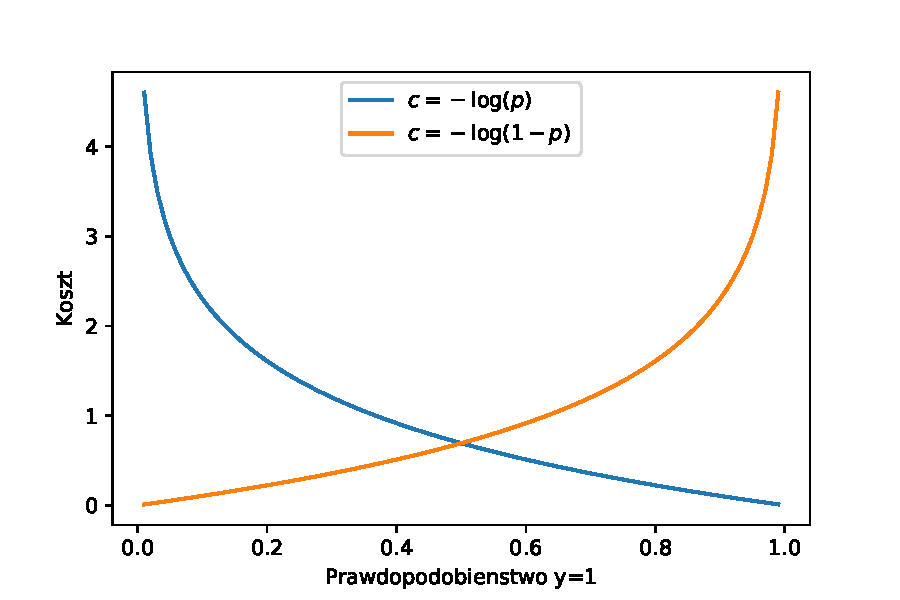
\includegraphics[width=\textwidth]{logreg-cost-single.pdf}
\end{frame}

\begin{frame}{Funkcja kosztu dla pojedynczego przykładu}
\begin{block}{Zadanie}
Zapisać poniższą funkcję jako pojedyncze wyrażenie (używając dodawania, mnożenia itp.):
\[ c(y, p) = \begin{cases} -\log(p) & y=1 \\ -\log(1-p) & y=0 \end{cases} \]
\end{block}
\note<1>
{
\[ c(y,p) = -y\log(p) - (1-y)\log(1-p) \]
}
\end{frame}

\begin{frame}{Funkcja kosztu dla całego problemu}
\begin{gather*}
\vec{p} = \sigma(\vec{X}\vec{w}) \\
J(\vec{w}) = \frac{1}{n} \sum_{i=1}^n c\left(y_i, p_i\right) = \\
-\frac{1}{n} \sum_{i=1}^n \left[ y_i\log p_i + (1-y_i)\log (1-p_i) \right] 
\end{gather*}
\pause
\[\frac{\dd J}{\dd w_i} = \frac{1}{n} \sum_{i=1}^n \left(\sigma(\vec{X_i}\vec{w})-y_i\right)X_{i,j} \]
\end{frame}

\begin{frame}{\emph{Softmax regression}/\emph{Multinomial logistic regression}}
\begin{block}{Zadanie klasyfikacji}
Dla danego wektora cech $x$ opisującego obiekt przewidzieć, do której z $K$ predefiniowanych klas należy obiekt: $y\in \{1, 2, \ldots, K\}$
\end{block}
% X n*p
% W p*k
\begin{gather*}
\vec{W} \text{ macierz wag typu } p\times k \\
\vec{P} \text{ macierz prawdopodobieństw typu } n\times k \\
\hat{\vec{P}} = \sigma(\vec{X}\vec{W}) = \left[ \frac{\sigma(\vec{X_{i,\cdot}}\vec{W_{\cdot,k}})}{\sum_{l=1}^K \sigma(\vec{X_{i,\cdot}}\vec{W_{\cdot,l}})} \right]_{i,k} \\
\hat{y_i} = \arg\max_{k} \hat{P_{i,k}} = \arg\max_{k} \vec{X_{i,\cdot}}\vec{W_{\cdot,k}} \\
\end{gather*}
\end{frame}

\begin{frame}{Uczenie regresji softmax}
\begin{gather*}
Y_{i,k}=\begin{cases} 1 & y_i=k \\ 0 & \text{w przeciwnym przypadku} \end{cases} \\
J(\vec{W}) = -\frac{1}{n} \sum_{i=1}^n \sum_{k=1}^K Y_{i,k}\log\hat{P_{i,k}} \\
\grad_{\vec{W_{\cdot,k}}} J(\vec{W}) = \frac{1}{n}\sum_{i=1}^n \left(\hat{P_{i,k}} - Y_{i,k}\right)\vec{X_{i}}
\end{gather*}
\end{frame}

\end{document}
